\section[Adaptive physics-based animation]{Adaptive techniques and models for physics-based animation}
\label{sec:starAdaptivity}
Complex real-world behaviors may exhibit multi-scale phenomena in space and time, large deformations or topological changes.
Sophisticated physical models involving a tremendous number of degrees of freedom are required to accurately reproduce these phenomena.
This comes at a high memory and computational price that can quickly become intractable or prevent from an interactive usage.
Adaptive models provide a general paradigm to solve these efficiency goals.
\\
We call a model or simulation method \emph{adaptive} if it automatically adapts the underlying mathematical representation, data structure and/or algorithm at run time, based on the evolving state of the simulated system.
The adaptation is designed for meeting a given criteria which depends on the application. 
Examples of frequently used criteria include reducing the overall computational complexity without loss of quality, improving the quality of real-time simulation, or simulating more precisely the parts of the scene with which the user is currently interacting.
\\
In this section, we review the different families of adaptive methods and present the way they have been applied in the different domains. In Section~\ref{sec t adaptivity}, we present time adaptive techniques such as dynamic time stepping and freezing techniques.
Then, we focus on spatially adaptive techniques.
Section~\ref{sec:spatial_refinement} discusses the most popular approach of spatial adaptivity: geometric adaptivity(\textit{h}-adaptivity where \textit{h} classically refers to the size of elements in the finite element method), which refers to varying the discretization resolution via refinement and coarsening strategies. This section is subdivided according to the types of adaptive spatial discretization.
Section~\ref{sec pr adaptivity} covers other spatial adaptivity approaches: basis refinement which adapts the number of bases, their order (\textit{p}-adaptivity where \textit{p} stands for polynomial), the basis functions themselves using enrichment, or, in subspace simulation, the deformation modes of the basis; moving grids methods (\textit{r}-adaptivity where \textit{r} stands for relocation) which relocate nodes without changing their connectivity; and mixed models which selectively apply a combination of different computational models. This organization reflects the taxonomy we propose in Figure~\ref{fig:taxonomy}.
We finally conclude and sketch future research avenues in adaptive simulation.
\\ \\
This section was published in journal \emph{Computer Graphics Forum, 2016}~\cite{Manteaux2016}.
\begin{figure}[!h]
	\centering
	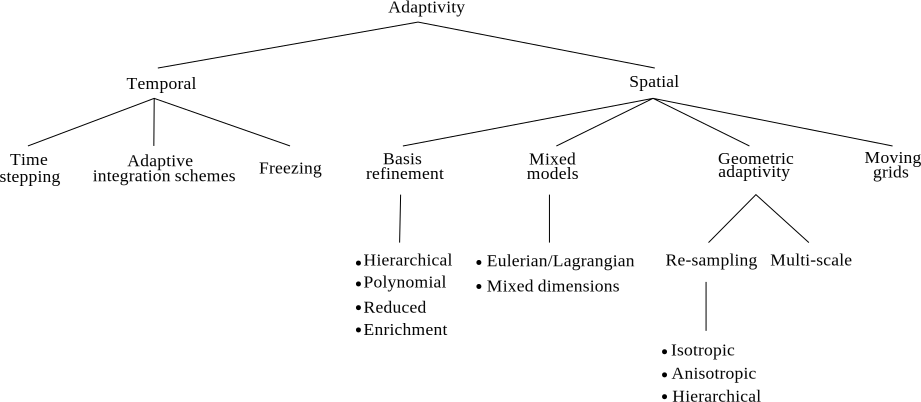
\includegraphics[width=\linewidth]{images/starAdaptivity-cgf2016/taxonomy.png}
	\caption[STAR adaptivity: Taxonomy]{\label{fig:taxonomy}Taxonomy of adaptive physically-based models in Computer Graphics. Temporal adaptivity (see Section \ref{sec t adaptivity}) and geometric adaptivity (see Section~\ref{sec:spatial_refinement}) are the two most common strategies. Basis refinement (see Section~\ref{sec:basis_refinement}), moving grids (see Section~\ref{sec:movingMesh}) and mixed models (see Section~\ref{sec:mixed-models}) are less common but proved to be very promising.}
\end{figure}

\subsection{Temporal adaptivity} \label{sec t adaptivity}
Animating any simulated object requires integrating its equations of motion over time.
There are many reasons why this integration procedure may need to adapt to the circumstances of the simulation, whether for accuracy, consistency, or stability.
For instance, a system entering a highly nonlinear regime, such as during fracture, typically requires smaller time steps to maintain the desired degree of accuracy.
Alternatively, adaptive time steps may be necessary to prevent the system from entering an invalid state: for example, many collision resolution schemes maintain the invariant that the system is never allowed to enter an interpenetrating configuration, which can require adjusting the time step according to the frequency of collisions.
Finally, the stability of continuum-mechanical simulations is closely tied to the relationship between the time step length, the spatial resolution, and the speed of propagation of information in the system, so if either of the latter change (in the presence of \emph{spatial} adaptivity or fast-moving flow) the time step must be adapted as well.
\\ \\
Techniques for temporal adaptivity fall into two main categories.
One approach focuses on time resolution, that is, how to choose an appropriate step length for time integration.
The second focuses on integration techniques themselves, seeking to switch between different integration schemes depending on the local context. This section explores both of these possibilities for temporal adaptivity.

\subsubsection{Adaptive time step selection}

\paragraph*{Time step criteria}
First, let us focus on the simulation of continuous media, like fluids and elastic solids, whose models are governed largely by hyperbolic partial differential equations.
Here the most prominent criterion for time step selection is the Courant-Friedrichs-Lewy (CFL) condition \cite{Courant1928}.
To understand this condition, we first note that the solution of a partial differential equation at some point depends on a particular subset of initial or boundary data; we call this subset of data the \emph{domain of dependence}.
The CFL condition states simply that for any numerical scheme to converge to the true solution, the domain of dependence of the numerical scheme must, in the limit, contain the true domain of dependence of the underlying differential equation.
(Otherwise, one could perturb the initial data in the region outside the numerical domain of dependence and change the true solution without affecting the computed one.)
The CFL condition can also serve as a stability criterion thanks to the Lax-Richtmeyer equivalence theorem \cite{Lax1956,Strikwerda2004}, which states that a consistent finite difference method for a well-posed initial value problem is convergent if and only if it is stable.
\\ \\
For example, for the classical wave equation $\partial_t^2 f = c^2\nabla^2 f$, the domain of dependence of any point $(\mathbf x, t)$ includes only points $(\mathbf x_0, t_0)$ with $\|\mathbf x-\mathbf x_0\|\le c(t-t_0)$, because information propagates only at the wave speed $c$.
Consequently, the time step $\Delta t$ must be small enough to prevent information from propagating outside the spatial stencil over a single time step.
In particular, for the first-order explicit finite difference scheme applied to the wave equation, where over each time step a grid cell is only affected by adjacent grid cells (separated by $\Delta x$), the CFL condition requires that $c\Delta t \le \Delta x$.
\\
In general, the CFL condition typically takes the form
\begin{align}
  \label{eq:cfl}
  C \equiv \frac{c\Delta t}{\Delta x} \le C_{\max},
\end{align}
where $c$ is the speed of information propagation, and $C_{\max}$ is a method-dependent constant which depends on the size of the finite-difference stencils.
The dimensionless ratio $C$ is known as the CFL number or the Courant number.
Note that implicit methods are not restricted by the CFL condition because the solution at any point at the end of the time step depends on the values at \emph{all} the points at the beginning of the time step, so the numerical domain of dependence is effectively infinite.
\\
The CFL condition can be a useful heuristic even in situations where it does not directly apply.
In computer graphics, semi-Lagrangian advection \cite{Stam1999} has been a popular scheme for solving the advection equation, as it is unconditionally stable and not restricted by the CFL condition \cite{Bridson2008}.
Nevertheless, excessively large time steps can lead to undesirable artifacts such as numerical dissipation and volume loss.
Foster and Fedkiw \cite{Foster2001} advocate limiting the time step size using \eqref{eq:cfl} with $c$ being the maximum of the flow speed $\|\mathbf u\|_\infty$ over the domain, and $C_{\max} = 5$.
\\
In Smoothed-Particle Hydrodynamics (SPH), each particle is affected by other particles within its smoothing radius $h$, analogous to the grid separation $\Delta x$ in finite-difference methods.
Consequently, time step selection criteria based on the CFL condition can be applied.
For pressure waves in compressible SPH, we continue to have
\begin{align}
  \label{eq:cfl_sph}
  \Delta t \le C_{\max}\frac hc,
\end{align}
and values of $C_{\max}$ between $0.25$ and $0.4$ have been used \cite{Monaghan1992,Desbrun1999}.
Fast relative motion of particles, which occurs especially during fluid-fluid or fluid-solid collisions, can also produce artifacts due to interactions not considered in \eqref{eq:cfl_sph}.
Therefore, one can introduce additional time step constraints based on the instantaneous acceleration $\mathbf a$ and divergence of velocity $\nabla \cdot \mathbf v$ \cite{Monaghan1992,Desbrun1999}:
\begin{align}
    \label{eq:acc_sph}
    \Delta t &\leq \Lambda \sqrt{\frac{h}{\|\mathbf a\|}}, \\
    \label{eq:div_sph}
    \Delta t &\leq \frac{\Gamma}{|\nabla \cdot \mathbf v|}.
\end{align}
$\Lambda$ and $\Gamma$ are dimensionless constants which Desbrun et al. \cite{Desbrun1999} set to $0.5$ and $0.005$ respectively.
Equation \eqref{eq:acc_sph} can in fact be interpreted as a CFL-type condition comparing the size of the spatial neighborhood, $h$, to a particle's relative displacement $\frac12\|\mathbf a\|\Delta t^2$ due to acceleration over time $\Delta t$.
Finally, we also point out that these criteria \eqref{eq:cfl_sph}--\eqref{eq:div_sph} may either be applied globally by taking the minimum of all particles' allowed time steps, or locally on a per-particle basis (as we discuss below).
\\
When adapting the time step based on higher-order derivatives such as acceleration \eqref{eq:acc_sph}, care must be taken because such quantities can be much noisier than the system variables themselves, causing large fluctuations in $\Delta t$.
Ihmsen et al.~\cite{Ihmsen2010} have observed that in incompressible SPH simulations, these time step fluctuations can lead to spurious density shocks that destroy the convergence of the simulation.
A solution is to change $\Delta t$ gradually rather than instantaneously: if the system violates any of the desired time step criteria, $\Delta t$ is decreased by a small amount (\cite{Ihmsen2010} use $0.2\%$), otherwise, if it is well within all the criteria, $\Delta t$ is increased by the same amount.
This strategy causes the time step to change smoothly towards the ideal step length.
On the other hand, it may also prevent the time step from changing quickly enough to resolve sudden shocks, such as those from high-velocity impacts.
Therefore, Ihmsen et al. introduce an additional procedure that detects shocks if the density error increases suddenly; if so, the simulation is rewound two time steps and resumed with a sufficiently small $\Delta t$.
\\ \\
Shock detection can be considered an example of an \textit{a posteriori} time step adaptation strategy, where undesirably large time steps are detected and rewound.
This kind of approach is useful whenever it is costly or difficult to estimate the right time step length in advance.
Instead, we simply perform a time step with the current estimate of $\Delta t$, and then test whether it adequately resolves the motion of the system.
If not, we reject the step, decrease the time step by setting $\Delta t\gets\Delta t/\alpha$ for some factor $\alpha>1$, and try again.
When several time steps in a row are successful, we increase the time step, $\Delta t\gets\alpha\Delta t$.
\\
Bridson et al.~\cite{Bridson2002} use this approach for efficient collision handling in cloth simulation, using a combination of inelastic repulsion forces and a robust collision resolution algorithm.
Inelastic repulsions are much more inexpensive than full collision resolution, but as they only check proximity at discrete points in time, they can easily fail to prevent interpenetrations if the cloth moves too far in a single time step.
If this happens, the time step is rejected and $\Delta t$ is reduced; collision resolution is only triggered if after multiple failures the time step falls to a specified minimum size.
The collision resolution step incorporates rigid impact zones \cite{Provot1997}, which can be seen as a freezing technique and is discussed in Section \ref{sec:adaptive-integration}.
Bargteil et al.~\cite{Bargteil2007} simulate plastic flow using a finite element mesh, where excessive deformation of elements can be problematic.
They reject a time step if any edge changes significantly in length, or a sudden acceleration takes place.
Both methods discussed here use $\alpha=2$, that is, time steps are halved or doubled as needed.
\\
The main drawback of this \textit{a posteriori} strategy is that the whole system must be globally rolled back to its previous safe state, even if it was caused by a localized event.
In rigid bodies simulation, this challenge was addressed by Mirtich \cite{Mirtich2000} to efficiently handle collisions.
Inspired by the work of Jefferson et al. \cite{Jefferson1985}, he proposed a \emph{time warp} algorithm to asynchronously handle collision events.
Here, the integration of a rigid body is interrupted only when resolving an event that concerns it.
This technique can be seen as a local time stepping technique, and inspired works on \emph{asynchronous variational integrators} (AVIs) which we discuss later in this section.

\paragraph*{Global time stepping}

The simplest way to perform adaptive time stepping is to choose the time step that is safe for the entire simulation domain, and perform integration for the entire system using that time step.
That is to say, given a time step criterion (or criteria) such as \eqref{eq:cfl_sph}--\eqref{eq:div_sph} that can be evaluated locally, one evaluates the permissible time step $\Delta t_i$ at all simulation points $i$, and steps the entire system forward by a time step of length $\Delta t = \min_i \Delta t_i$.
For methods that use implicit integration or other globally coupled schemes, such as grid-based fluids with a global pressure solve, this is typically the only possible approach.
For this reason as well as for its conceptual and practical simplicity, global time stepping is probably the most widely used form of temporal adaptivity in practice.
\\
It is worth pointing out here that adaptive time stepping is not a free lunch for all time integration schemes.
The Verlet, or leapfrog, scheme is second-order accurate, and has excellent energy conservation properties thanks to its symplectic nature, but both these features rely on the time step being fixed.
To maintain second-order accuracy with a variable time step, Bridson et al. \cite{Bridson2003} proposed a time integration scheme that combines a leapfrog scheme for position with an implicit trapezoidal rule for velocity:
\smallskip
\begin{algorithmic}[1]
\State $\tilde v^{n+1/2} = v^n + \frac{\Delta t}2 a(t^n, x^n, \tilde v^{n+1/2})$ \Comment implicit
\State $x^{n+1} = x^n + \Delta t\tilde v^{n+1/2}$ \Comment explicit
\State $v^{n+1/2} = v^n + \frac{\Delta t}2 a(t^n, x^n, v^n)$ \Comment explicit
\State $v^{n+1} = v^{n+1/2} + \frac{\Delta t}2 a(t^{n+1}, x^{n+1}, v^{n+1})$ \Comment implicit
\end{algorithmic}
Maintaining symplecticity is much more challenging, as naively varying the time step can lead to instabilities and inconsistent energy behavior~\cite{Harmon2009}.
Much more elaborate time stepping schemes are needed to recover energy preservation, such as the asynchronous variational integrators discussed below.

\paragraph*{Local time stepping}
In complex simulation scenarios, different regions of the simulation domain may have very different time step requirements.
For example, resolving challenging collision and contact scenarios requires careful time stepping, but only for the parts of the system that are affected by the contact.
Similarly, in simulations with adaptive spatial resolution, the CFL condition requires finer-resolution regions to take smaller time steps.
It can become intractable to simulate the whole model in lockstep using the most conservative time step.
Instead, it is desirable to perform local time stepping, integrating each element of the simulation at its own pace.
\\
Explicit integration schemes can readily incorporate local time stepping.
We illustrate this with a generic two-dimensional system,
\begin{align}
  q_1'(t) &= f_1\big(t, q_1(t), q_2(t)\big), \\
  q_2'(t) &= f_2\big(t, q_1(t), q_2(t)\big).
\end{align}
If at time $t$, $q_2$ requires a very small time step $\Delta t_2$, one can still integrate $q_1$ with its own time step $\Delta t_1$, giving
\begin{equation}
  q_1(t+\Delta t_1) = q_1(t) + \Delta t_1 f_1\big(t, q_1(t), q_2(t)\big).
\end{equation}
Meanwhile, as $q_2$ takes multiple steps to cover the same time interval, it will require values of $q_1$ at intermediate times $t+\Delta t_2$, $t+2\Delta t_2$, and so on; these can be linearly interpolated from $q_1(t)$ and $q_1(t+\Delta t_1)$.
Equivalently, to simplify bookkeeping, one can take the same small time steps $\Delta t_2$ for both $q_1$ and $q_2$, but only evaluate $q_1'$ at the first step and hold it fixed until a time $\Delta t_1$ has been covered.
This approach has the same computational advantage because evaluation of $f$ is typically the most expensive part in explicit methods.
\\
Early work on SPH \cite{Desbrun1996,Desbrun1999} recommended this approach for local time stepping, using the CFL condition as the time step criterion.
The same technique was also used to simulate elastic bodies using spatially adaptive finite element meshes \cite{Debunne2001}, discussed in more detail in Section \ref{sec:meshes}.
For a linear elastic material with density $\rho$ and Lam\'e coefficients $\lambda$ and $\mu$, the upper bound on the time step for an element can be approximated by
\begin{equation}
  \label{eq:cfl-fem}
  \Delta t \le h\sqrt{\frac\rho{\lambda+2\mu}}
\end{equation}
where $h$ is a measure of the size of the element, such as its inradius: skinnier elements or stiffer materials require smaller time steps.
To improve the parallelization of local time stepping for SPH fluids, Goswami and Batty \cite{Goswami2014} divide the computational domain into blocks and choose time steps independently per block.
\\ \\
Asynchronous variational integrators (AVIs) studied by Lew et al. \cite{Lew2004} are a family of time integration schemes that provide excellent energy conservation behavior while allowing different elements of the system to use different time steps.
Unlike the local time stepping model described above, AVIs associate a time step with each \emph{force} rather than each variable.
Thus each force term applies a series of impulses to its associated nodes.
The time step for a particular term must remain constant throughout the simulation, but different forces may have very different time steps.
This approach is typically implemented as an event-driven simulation loop, using a priority queue to schedule the updates for all the forces in order.
Thomaszewski et al. \cite{Thomaszewski2008} applied this approach to cloth simulation with a finite element triangle mesh, choosing time steps independently for each element using the CFL criterion \eqref{eq:cfl-fem}.
AVIs are known to exhibit ``resonance instabilities'' that can potentially cause the energy to increase without bound; however, these instabilities tend to be extremely weak in solid mechanics problems \cite{Fong2007} and have not been observed to cause difficulties in computer graphics \cite{Harmon2009}.
\\
The energy conservation properties of AVIs hinge on the regular spacing of the impulses applied by each force term, which makes collisions challenging to incorporate: naively applying contact forces at the moment of collision breaks the periodicity and destroys energy conservation, while applying contact forces at regular intervals risks missing collisions.
Recent work \cite{Harmon2009,Ainsley2012} addresses this problem by replacing each contact force with a sum of stiffer and stiffer penalty layers with smaller and smaller time steps, which together are guaranteed to prevent interpenetration.
While the number of penalty layers is conceptually infinite, any given collision can only activate a finite number of penalty layers, so the actual amount of computation is finite.
Initial work by Harmon et al.~\cite{Harmon2009} used kinetic data structures to detect all collision events in advance.
Ainsley et al.~\cite{Ainsley2012} instead adopt a speculative approach based on the time warp algorithm \cite{Jefferson1985, Mirtich2000}, analogous to the \textit{a posteriori} time step adaptation techniques discussed previously.
An interval of time is first simulated without considering any new collisions; then, collision detection over the simulated interval is performed, and if new collisions are found, those force terms are activated and the interval is re-simulated.
Speculative simulation greatly reduces the computation time spent in bookkeeping and collision detection, and also allows for easy parallelization.

\subsubsection{Adaptive integration}
\label{sec:adaptive-integration}

\paragraph*{Adaptive choice of time integration scheme}
In some cases, such as when the system involves highly stiff modes or poorly conditioned elements, an adaptive choice of time step is no longer the most efficient strategy.
The time step requirements for explicit integration may become extremely restrictive.
Instead, one may locally change the integration scheme to deal with the problematic components, for example by switching to an implicit method or a nonlinear one.
By doing so adaptively, one can continue to use an inexpensive explicit integration scheme for the remainder of the system.
\\
In the finite element method, ill-shaped elements impose severe restrictions on the allowed time step for explicit integration \eqref{eq:cfl-fem}.
When the object undergoes topological changes such as cutting or fracture, it can be difficult to avoid introducing such elements.
As an alternative to local time stepping, where ill-shaped elements would have to be simulated with extremely small time steps, Fierz et al. \cite{Fierz2011} propose an element-wise implicit-explicit (IMEX) scheme.
Here the same time step $\Delta t$ is used for the entire system, but ill-shaped elements that would be unstable if explicitly integrated over $\Delta t$ are instead simulated with an unconditionally stable implicit scheme.
Nodes that are not adjacent to any ill-shaped element are integrated explicitly, then held fixed as boundary conditions for implicit integration of the remaining nodes.
As long as the number of ill-shaped elements is low, this relaxes the time step restriction faced by explicit integration, while minimizing the computational cost and numerical dissipation associated with implicit integration.
\\
Thin materials such as hair exhibit a high stiffness in their stretching modes, but pose the additional challenge that their collision response is highly nonlinear due to the presence of rotation.
Therefore, depending on the amount of bending, an implicit first-order model for collisions may fail to capture the correct response and lead to instabilities.
Kaufman et al. \cite{Kaufman2014} propose an algorithm that adaptively chooses the \emph{degree} of nonlinearity in each contact resolution step to safely resolve the collision.
Specifically, they adapt the number of constrained Newton iterations used to solve the nonlinear contact model, terminating when the stretch over all affected edges is sufficiently reduced.
This allows for large simulation time steps in the face of many energetic collisions, while efficiency is maintained because most collisions require only a single iteration (equivalent to a linearly implicit step).

\paragraph*{Freezing techniques}
Freezing techniques, also called sleeping techniques, lie in between temporal and spatial adaptability: the degrees of freedom that are considered unimportant in the simulation are kept constant in time for a specified duration.
This can be seen as animating them at a much larger time scale, or as temporarily deactivating them.
No memory is saved while doing so, but computation time is reduced.
These techniques are useful in situations where the spatial domain is large and filled with many quiescent objects.
Therefore, game environments and surgical simulations are perfect candidates for these methods.
Conversely, freezing techniques may not be useful in highly dynamic situations where most of the degrees of freedom are active most of the time.
In addition to defining good freezing criteria, the main challenge of freezing techniques is to design a reactivation process of the frozen degrees of freedom that ensures plausible subsequent motion.
\\
In rigid objects simulation (see the survey of Bender et al. \cite{Bender2012:rigid}), important computational resources are dedicated to solving contacts between the different objects of a scene.
This process becomes unnecessarily expensive when stacking occurs and nothing moves.
In these cases, freezing techniques prove to be useful for saving computational time without compromising the plausibility of the simulation.
\\
Schmidl \cite{Schmidl2002} uses a heuristic based on kinetic energy to determine whether to freeze a body or not:
\begin{equation}
\label{eq:shmidl_freezing}
\frac{1}{2}m\mathbf{v}^{2} + \frac{1}{2}\mathbf{\omega}^{T}\mathbf{I}\mathbf{\omega} < \frac{\mathbf{p}_{g}^{2}}{2m}
\end{equation}
where $\mathbf{v}$ and $\mathbf{\omega}$ respectively denote the linear and angular velocity of the rigid body of mass $m$ and inertia tensor $\mathbf{I}$, and $\mathbf{p}_{g}=m\mathbf{g}\Delta t$ is the momentum that the body accumulates during a time step $\Delta t$ from gravity.
If condition \eqref{eq:shmidl_freezing} is fulfilled by the body during a user-defined number of consecutive time steps, then it is frozen.
Note that a single frozen body by itself does not save computation time.
Time is saved when multiple neighboring objects become frozen, as their contact forces no longer need to be computed.
The only way for a frozen rigid body to be reactivated is when it receives a large impulse during a collision.
Once it is reactivated, the information is propagated to all its direct neighbors and a given number of indirect neighbors, potentially awakening them (see Figure \ref{fig:stackFreezing}).
\begin{figure}[!h]
	\centering
	\begin{subfigure}[b]{0.45\linewidth}
		\centering
		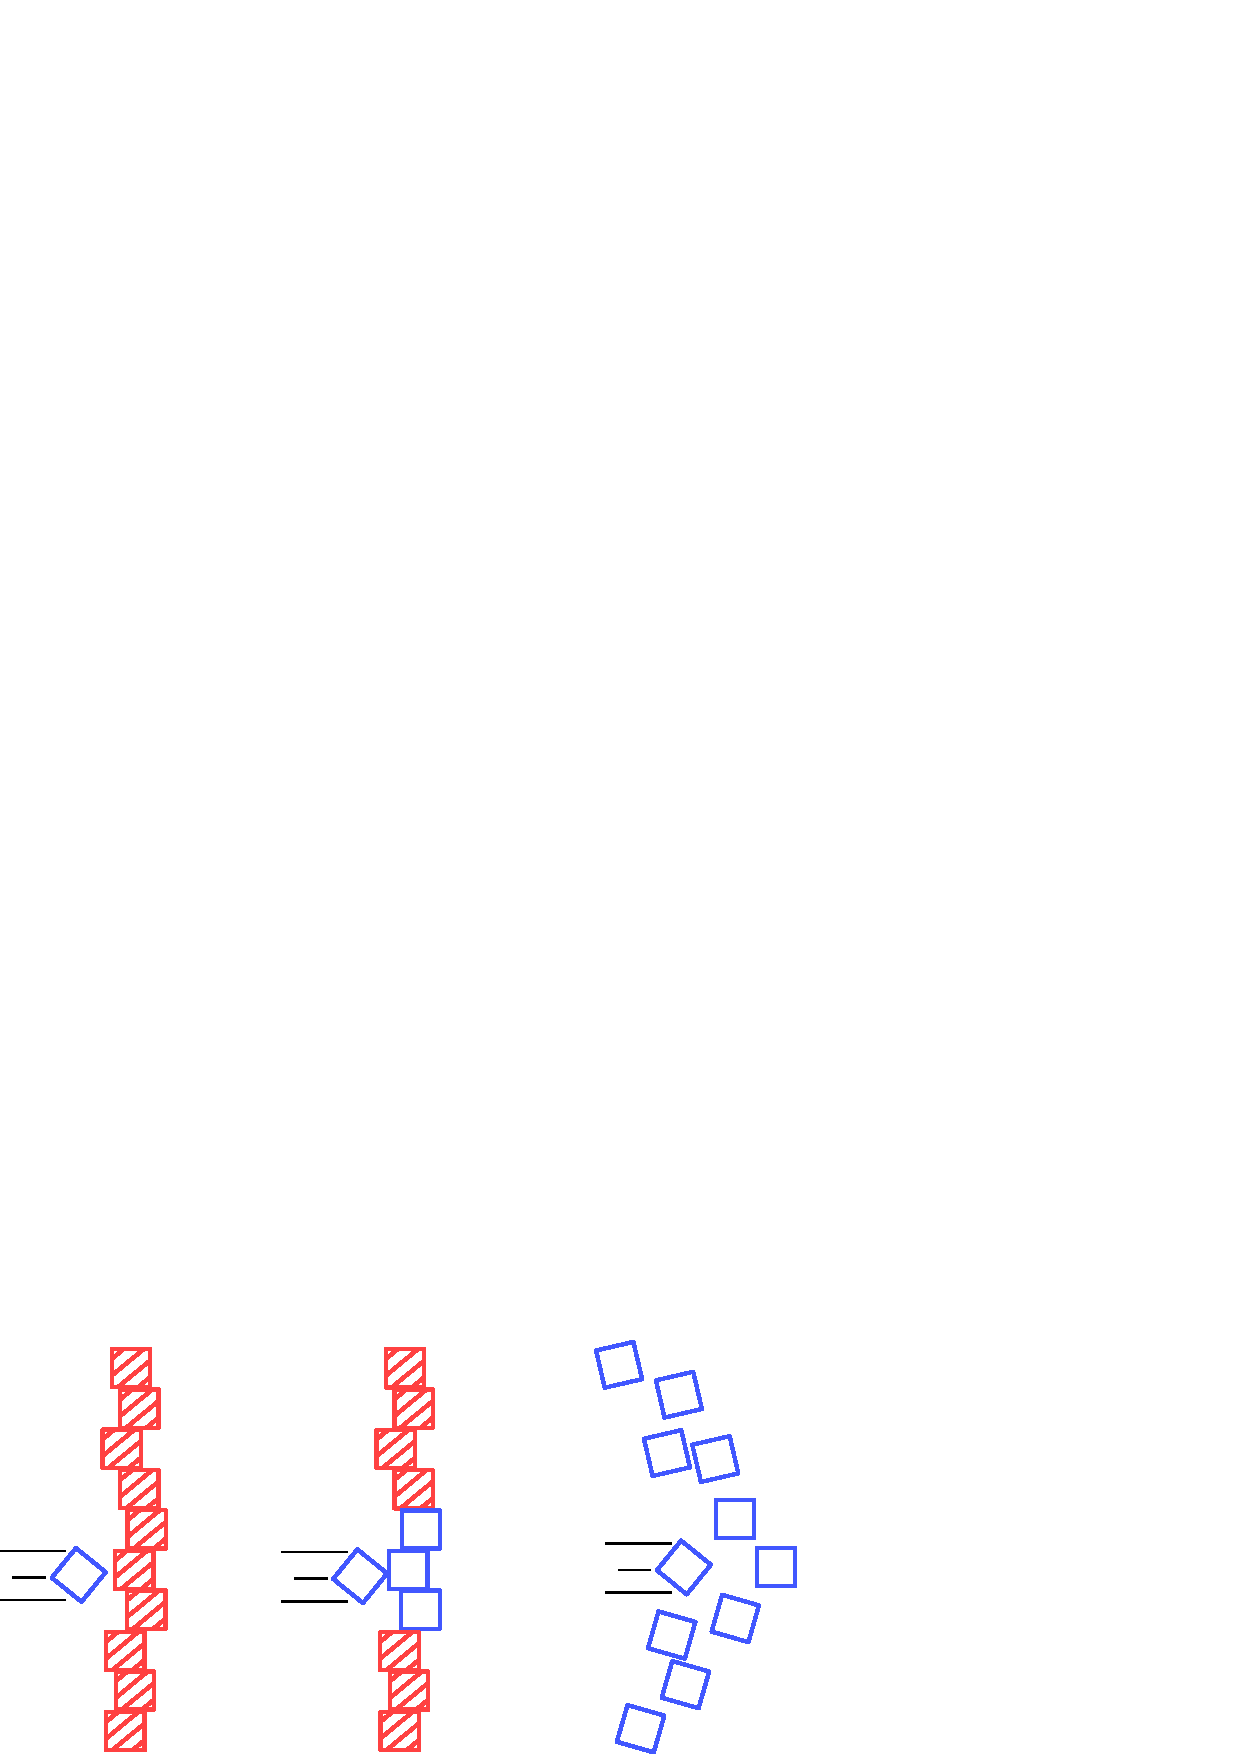
\includegraphics[scale=0.5]{images/starAdaptivity-cgf2016/freezing-rigid.png}
		\caption{\label{fig:stackFreezing}}
	\end{subfigure}
	\hfill
	\begin{subfigure}[b]{0.45\linewidth}
		\centering
		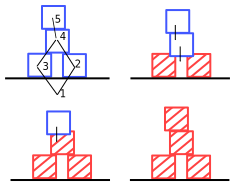
\includegraphics[scale=0.7, angle=0]{images/starAdaptivity-cgf2016/freezing-graph.png}
		\caption{\label{fig:graphFreezing}}
	\end{subfigure}
	\caption[STAR adaptivity: Rigid body freezing]{
		\label{fig:freezingTechniques}
		Freezing techniques applied to rigid bodies stacking. At the stage of contact solving, those methods can save computational time while ensuring a plausible motion.
		In (a), quiescent rigid bodies are frozen (in hatched red) in a stacking configuration. A collision event then awakes one of the rigid bodies, and the active rigid body (in blue) propagates the information to its neighbors.
		In (b), a contact graph stores stack ordering. During shock propagation, a bottom-up traversal is performed and objects at each level are frozen by assigning an infinite mass.
	}
\end{figure}
\\
Freezing techniques have been used as a failsafe procedure for resolving collisions and contact between rigid or deformable bodies.
When many interacting contacts are present, iterative processes for collision response can require an excessively large number of iterations to converge, and early termination leaves the system in an interpenetrating state.
Freezing procedures are attractive in this context as they can guarantee elimination of interpenetrations.
However, they also introduce loss of kinetic energy by treating contacts as fully inelastic, and are therefore only invoked as a last resort after multiple iterations of a physically correct solver have failed to resolve the collisions.
For rigid body contact, Guendelman et al. \cite{Guendelman2003} propose a shock propagation strategy which freezes bodies progressively from the ground up.
They start by building a directed acyclic graph consisting of ``levels'' of objects that are resting on objects of lower levels (cyclic dependencies are grouped into the same level).
A single bottom-up traversal of the graph resolves contacts level by level, assigning infinite mass to lower-level objects for which contact is solved (see Figure \ref{fig:graphFreezing}).
Rigid impact zones, described by Provot \cite{Provot1997} and Bridson et al. \cite{Bridson2002}, are extensively used to resolve collisions in cloth.
Nodes involved in multiple interfering collisions are collected into disjoint sets called ``impact zones'', constructed by merging zones if their nodes are involved in the same node-face or edge-edge collision.
Each impact zone is made rigid by replacing the motion of its nodes with a rigid body motion while preserving the total linear and angular momentum.
This process eliminates collisions within the zone, but may introduce new collisions with nearby elements outside the zone.
Therefore, one must perform collision detection again and grow the impact zones if new collisions are detected, iterating this process until no new collisions occur.
\\ \\
Freezing techniques were also used for articulated rigid bodies, both for dynamics~\cite{Redon2005} and quasi-statics~\cite{Redon2006}: joints are activated or deactivated based on user-defined error metrics, leading to a simplification of the whole model and a sub-linear computational complexity.
\\
Denoting by $\mathbf{\ddot{q}}^C=(\mathbf{\ddot{q}}_1,\ldots,\mathbf{\ddot{q}}_{N_C})^T$
the composite acceleration of an articulated body $C$, where $N_C$ is the number of joints in $C$, the \emph{acceleration
metric value} of $C$ is defined as
\[\mathcal{A}(C)=\sum_{i\in C}\mathbf{\ddot{q}}_i^T\mathbf{A}_i\mathbf{\ddot{q}}_i,\] where $\mathbf{A}_i$, $i\in C$, are symmetric, positive definite $d_{J_i}\times d_{J_i}$ \emph{weight matrices}, and $d_{J_i}$ is
the number of degrees of freedom of joint $i$ in $C$. The weight matrices $\mathbf{A}_i$ are required to depend at most on joint positions, and the simplest choice is the identity
matrix. The key to the sub-linear complexity is the demonstration that the acceleration metric of each sub-articulated body is a quadratic function of the forces applied to its handles (i.e. the free rigid bodies used to assemble sub-articulated bodies in Featherstone's methodology~\cite{Redon2005}). As a result, the acceleration metric may be computed \emph{before computing the joint accelerations themselves}. This is used during the top-down pass of Featherstone's divide-and-conquer algorithm to determine which joint accelerations should be computed because they are sufficiently large~\cite{Redon2005}. For example, if the acceleration metric of the complete articulated body is small, then all joint accelerations are small and joint velocities are constant for the current time step. A similar metric is built for joint velocities to determine which joint positions should remain constant, and thus which inter-body forces and inertial terms should be updated. Once all position-dependent terms are up to date, the motion metrics are available for the next time step, and a new set of active joints can be determined.
\\
It was shown that this approach could also help to speed up continuous collision detection for articulated bodies~\cite{Kim2008Collision} and haptics rendering~\cite{Morin2007}, as well as enable view-dependent articulated-body dynamics by combining motion metrics with visibility estimates~\cite{Kim2008View} (see Figure \ref{fig:ViewDependentArticulatedBodies}).
\begin{figure}[!h]
	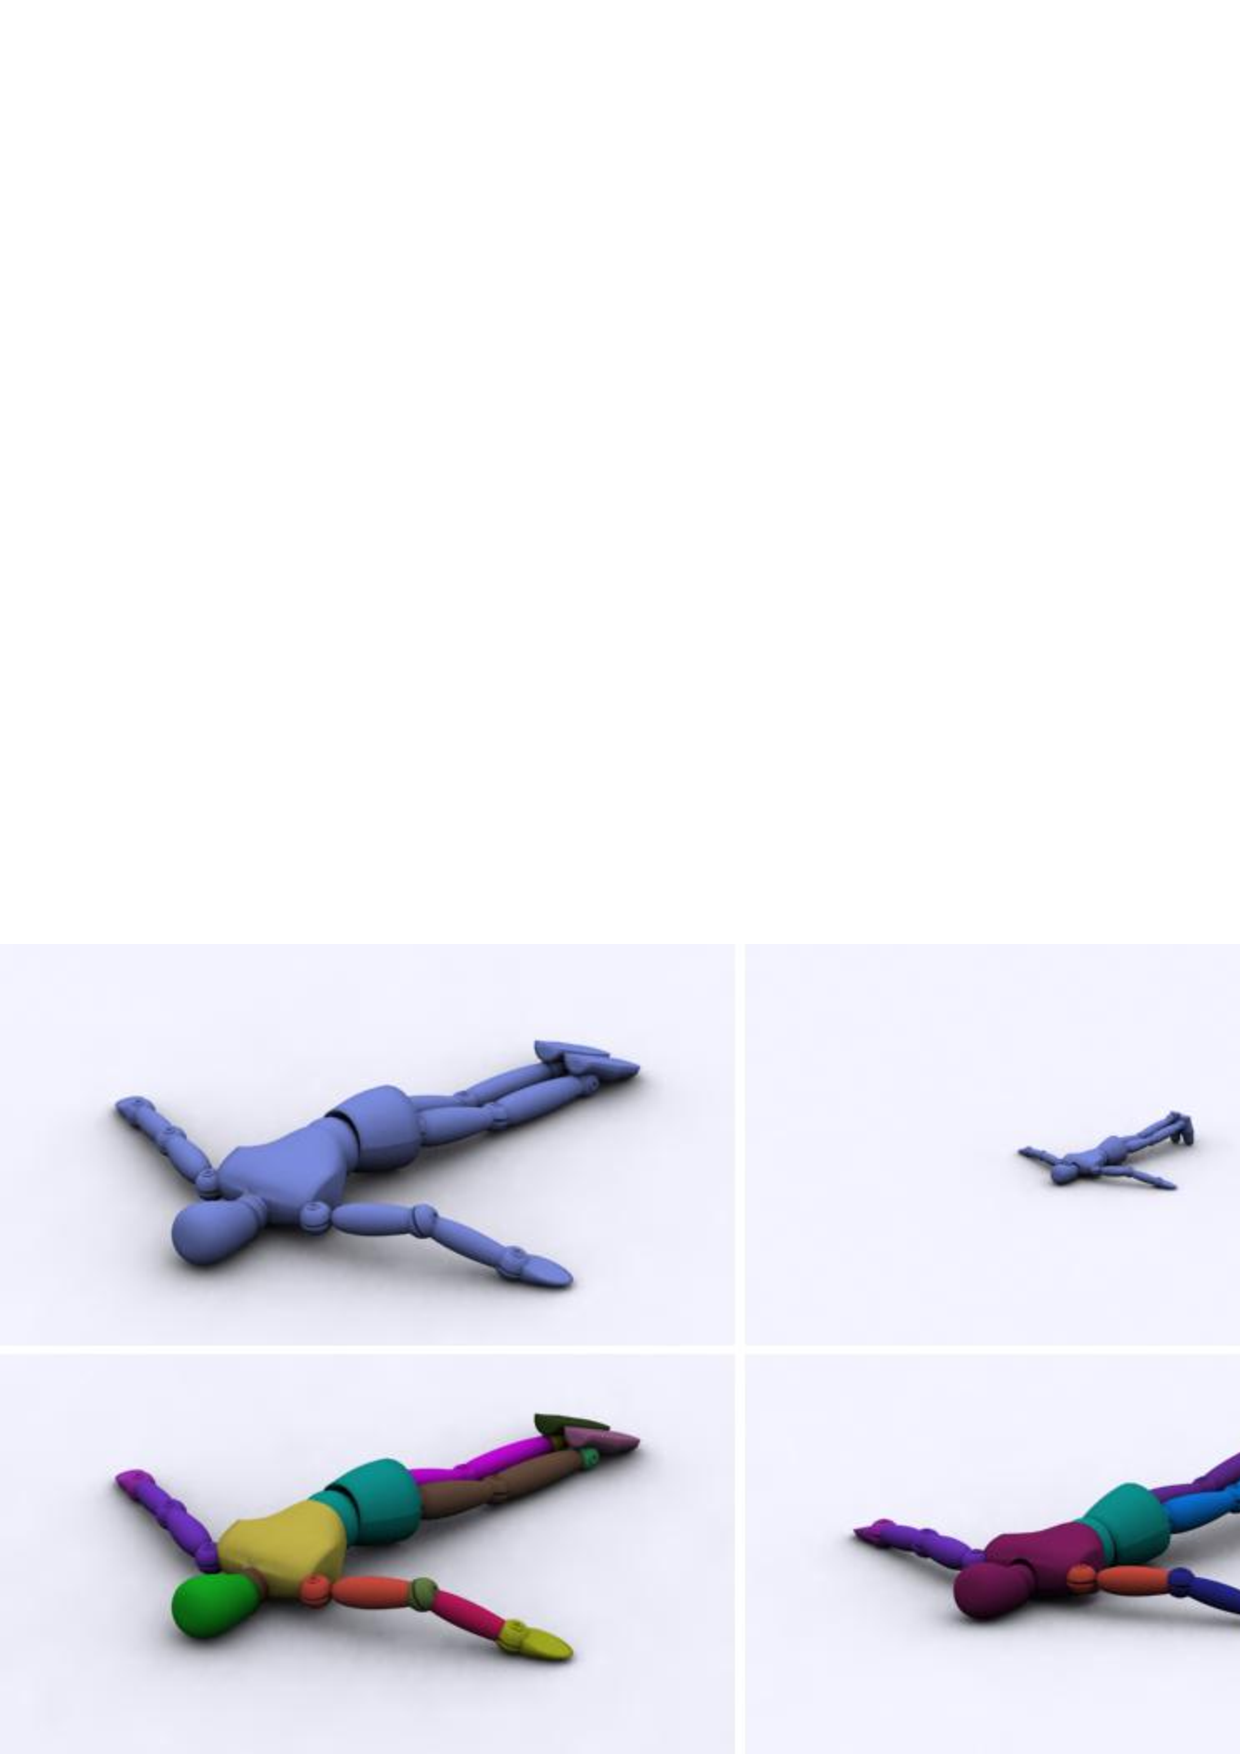
\includegraphics[width=\linewidth]{./images/starAdaptivity-cgf2016/WMComparisonNoLabels.png}
	\caption[STAR adaptivity: Articulated rigid body freezing]{\label{fig:ViewDependentArticulatedBodies}View-dependent dynamics of articulated bodies. Top: the algorithm proposed by Kim et al. \cite{Kim2008Collision} automatically simplifies the dynamics of a falling character as its distance to the viewer increases. Bottom: corresponding rigidification at this time step (one color per rigid group).}
\end{figure}
Gayle et al. \cite{Gayle2006} demonstrate how to perform contact handling with such an adaptive articulated-body method, which is used as the core of a physics-based sampling algorithm for highly articulated chains~\cite{Gayle2007} and cable route planning~\cite{Kabul2007}.
\\ \\
Recent work has sought to apply freezing techniques to accelerate SPH fluid simulation.
In these methods, particles are divided into two sets: a set of \emph{active} particles following a classical simulation step, and a set of \emph{inactive} particles that are skipped in the simulation.
As physical quantities in SPH are interpolated from neighbors, inactive neighbors of active particles also need to be updated to ensure that active particles compute correct physical quantities.
Computation time is saved for inactive particles that only have inactive neighbors.
The main challenge in these methods is the definition of the process to transform a particle from the inactive set to the active one and vice versa.
Indeed, as SPH is sensitive to particle distribution, an inadequate transition of state can directly lead to instabilities.
Additionally, a judicious choice of criterion to decide whether a particle should be active or not is essential.
\\
Goswami and Pajarola \cite{Goswami2011} propose a simple method that evaluates the active status of particles at each time step.
Particles are marked as active if they are close to the boundary or if their velocity exceeds a threshold.
Inactive neighbors of such particles are also added to the active set, and continue with their last active velocity.
All other particles are considered inactive.
Unfortunately, the resulting method does not obey Newton's third law, resulting in some loss of momentum.
In the context of molecular simulation, Artemova and Redon \cite{Artemova2012} propose a fundamentally different approach which ensures momentum conservation. In Chapter~\ref{chap:arps}, we extend their work to computer graphics.

\subsection{Geometric adaptivity} 
\label{sec:spatial_refinement}

Geometric adaptivity describes various techniques that adapt the spatial resolution of a model by refining and coarsening its discretization. These techniques are also referred in the literature as \emph{adaptive spatial refinement}. However, as they include coarsening as well, we adopted a more general term.

Geometric adaptive techniques have two major components: a refinement criterion that determines where higher resolution is needed, and a refinement/coarsening scheme that modifies the discretization to match the desired resolution.
Both physical and visual criteria have been employed in existing work, and we discuss them in more detail below.
The refinement scheme itself essentially depends on the type of spatial discretization.
In the following subsections, we will deal with the three major kinds of discretization separately: structured meshes and grids, unstructured meshes, and meshless models.


\paragraph*{Refinement criteria}
The choice of refinement criteria plays a major role in the quality of the resulting simulation.
Many techniques use simple heuristics such as the distance to boundaries, surface curvature, and the presence of contacts.
However, some authors have shown that employing criteria that are more closely tied to the dynamics of the system can be important in many contexts.
\\
In elastic and plastic solids, the stress and strain in an element characterize the amount of local deformation.
Therefore, the values and gradients of these quantities are often used to control refinement.
Wu et al. \cite{Wu2001} describe several different error estimators of this type and discuss their relative advantages, drawbacks, and performance.
Going beyond estimating a scalar error, Wicke et al. \cite{Wicke2010} define a metric tensor $\mathbf M$ that approximates the spatial variation of strain by comparing deformation gradients of adjacent elements.
The matrix $\mathbf M$ is defined in such a way that it has large eigenvalues in directions in which the deformation changes most rapidly, and can thus be used to control anisotropic refinement (see Figure \ref{fig:Wicke2010}).
\begin{figure}[!h]
  \centering
  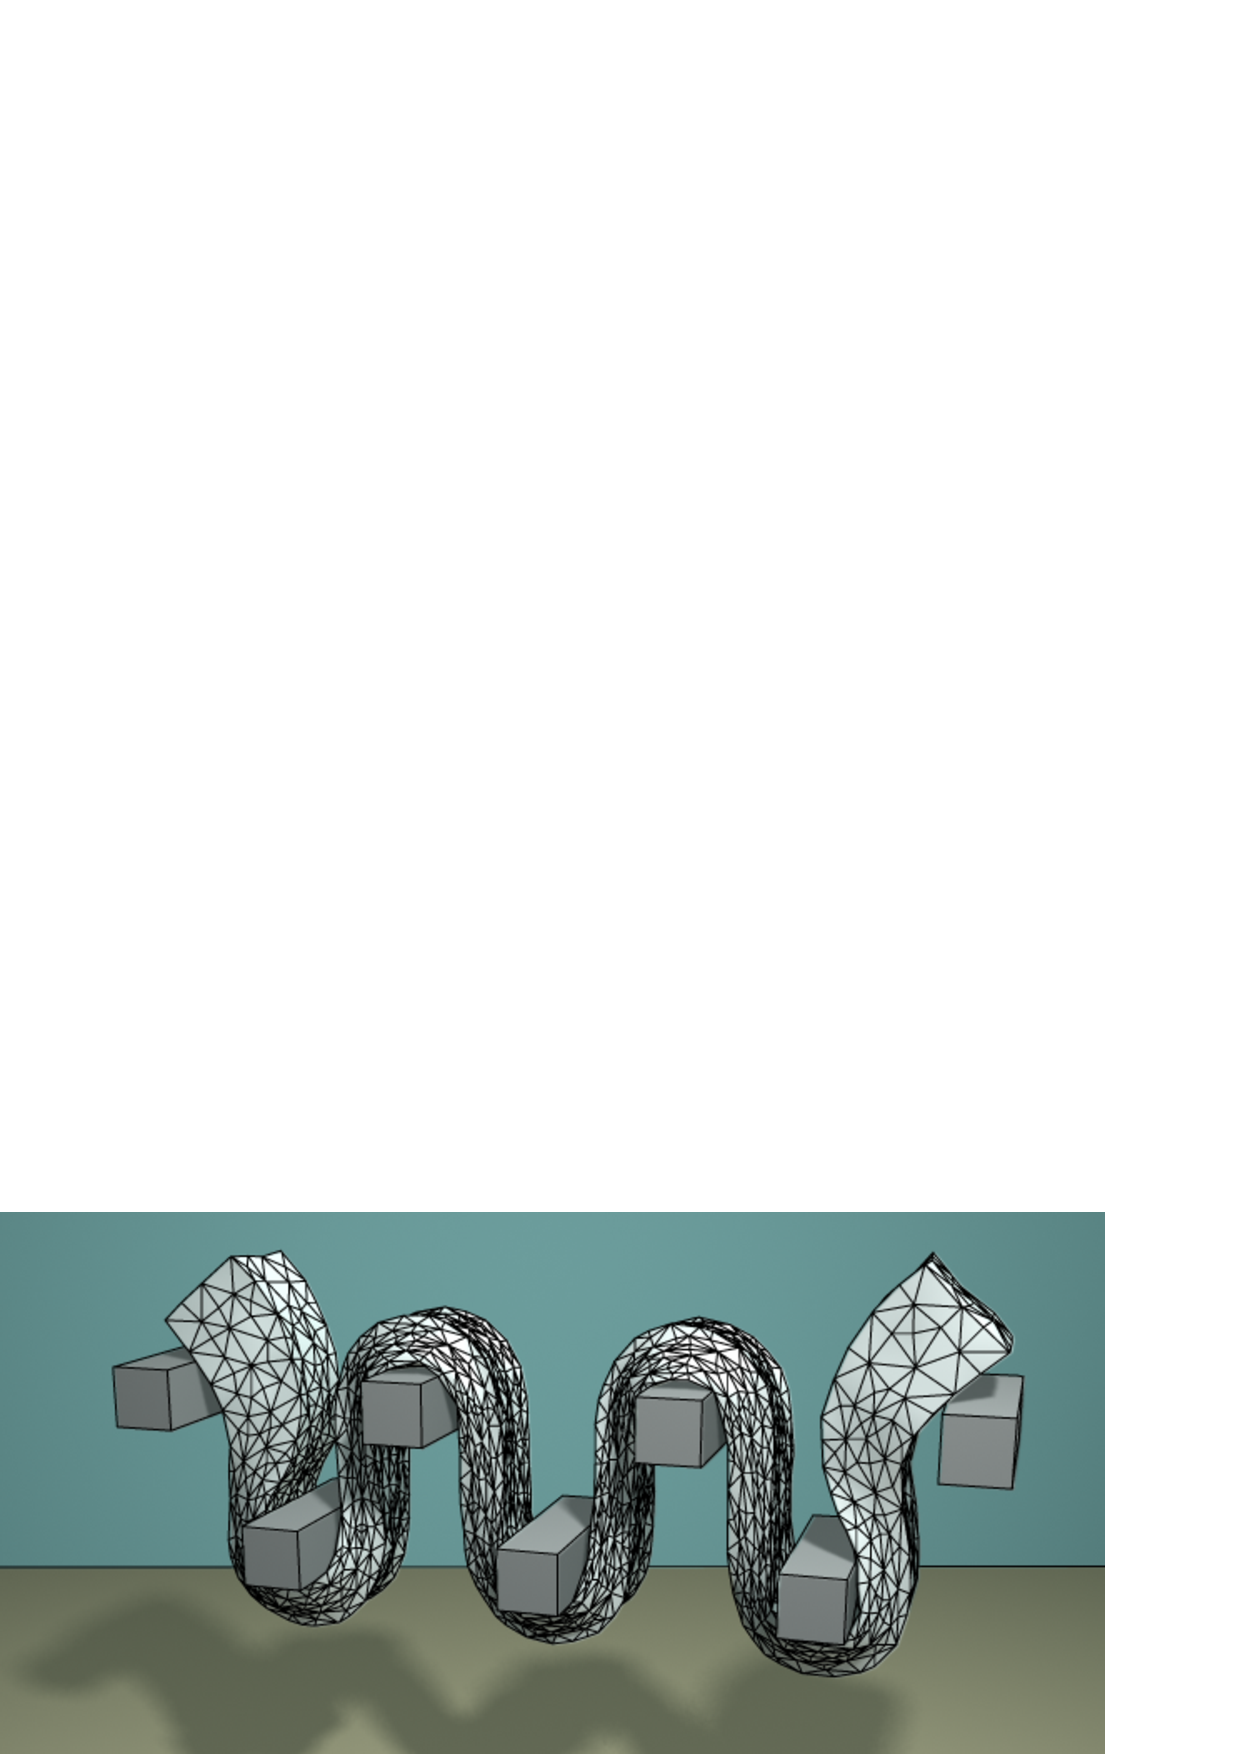
\includegraphics[width=0.8\linewidth]{images/starAdaptivity-cgf2016/mesh-plastic.png}
  \caption[STAR adaptivity: Tetrahedral remeshing]{Elastoplastic simulation with dynamic local remeshing \cite{Wicke2010}. By using the strain gradient as the refinement criterion, regions undergoing severe deformation are refined locally.}
  \label{fig:Wicke2010}
\end{figure}
\\
If a multi-grid algorithm is used, the difference between the solution at the current level, $\mathbf x^j$, and the one prolonged from the next coarser level, $\mathbf P^j\mathbf x^{j+1}$, provides a natural measure of the quality of $\mathbf x^{j+1}$.
Otaduy et al. \cite{Otaduy2007} weigh the error by the local system matrix $\mathbf A$ to reduce possible popping in stiff scenarios, leading to the error metric
\begin{equation}
	e = \|A^j(\mathbf x^j-\mathbf P^j\mathbf x^{j+1})\|,
\end{equation}
and perform refinement if $e$ exceeds a predefined threshold.
\\
Lower-dimensional bodies, like wires, strands, cloth, and thin sheets, undergo not just stretching but also bending (and torsion, in the case of one-dimensional strands).
While the stretching forces within the material are much stiffer than the bending forces, the bending deformation can often be more visually important, and also introduces geometric nonlinearities that must be carefully resolved.
In this context, geometrical curvature and the presence of contacts (which are likely to induce bending) are the most commonly used refinement criteria.
However, the interaction between stretching and bending leads to additional considerations.

First, in the context of cloth simulation, Simnett et al. \cite{Simnett2009} and Narain et al. \cite{Narain2012} point out that elements under compression are likely to buckle and should therefore also be refined, otherwise the wrinkles that would arise in subsequent time steps will fail to be represented on the coarse mesh.
By considering the trade-off between bending and stretching energy, Narain et al. estimate that a sheet under compressive strain $\epsilon$ is likely to form wrinkles of width proportional to $\sqrt{k_b/(k_s\epsilon)}$ where $k_b$ and $k_s$ are the bending and stretching stiffnesses respectively, providing an estimate of the extent of refinement necessary.
In the physics literature, Cerda and Mahadevan \cite{Cerda2003} have provided a detailed semi-analytical analysis of wrinkle geometry that is valid far from the small-deformation limit, and may be useful for future work in graphics.

Second, finer meshes allow higher-frequency modes of transverse oscillation, leading to time step constraints and stability problems that can be fatal for interactive applications.
To ensure stability, Servin et al. \cite{Servin2008} propose a \emph{coarsening} criterion, reducing the resolution of the mesh so that only those oscillations whose frequency is lower than the time stepping rate can be represented.
For simulation of systems with stiff wires, they estimate the maximum frequency of oscillations in a wire discretized with $n$ nodes as
\begin{equation}
	\omega_{\max} \approx 2(n+1)\sqrt{\frac{f}{mL}},
\end{equation}
where $f$ is the tension in the wire and $m$ and $L$ are its mass and length.
Requiring this frequency to be lower than $1/\Delta t$ gives an upper bound on $n$ for each wire.

In fracture simulation, the stress forms a singularity at the crack tip, which must be resolved accurately with a fine resolution mesh for realistic crack paths to be obtained.
If the crack origin is known \textit{a priori}, one can track the crack path as the fracture proceeds and refine the mesh based on the distance from the crack \cite{Busaryev2013}.
However, if fracture is allowed to originate anywhere, it is necessary to refine the mesh wherever stress is sufficiently high, i.e. close to the material's strength $\tau$, because such regions may generate new cracks.
Koschier et al. \cite{Koschier2014} refine elements whose tensile stress $\sigma$ exceeds a specified fraction of $\tau$.
Pfaff et al. \cite{Pfaff2014} choose the desired resolution of the mesh to be proportional to tensile stress by requiring the length of each edge $\mathbf e$ to satisfy
\begin{equation}
	\|\mathbf e\|\le\max\left(\frac{\tau}{2\sigma},1\right)\ell_{\min}
\end{equation}
where $\ell_{\min}$ is a user-specified refinement limit.
This approach allows the mesh to be coarsened again after the crack tip has passed.

It is also possible to perform view-dependent adaptivity by modulating the refinement criteria based on visibility and distance from the camera. Such techniques have been applied to the simulation of wires \cite{Servin2008} and cloth \cite{Koh2014}. New issues arise in such contexts, such as preventing artifacts when coarser regions come into the field of view and must be refined: Koh et al. \cite{Koh2014} achieve this by smoothly increasing the resolution in advance based on the known camera path.

Many adaptive methods for simulation of liquids have relied on the distance to the free surface as the sole refinement criterion.
However, much greater adaptivity is possible by observing that in regions where the surface is flat and does not exhibit detailed motion, it can also be coarsened without significantly affecting the flow.
Adams et al. \cite{Adams2007} propose a purely geometrical criterion based on an ``extended local feature size'' which measures the distance to the surface and to the medial axis of the fluid volume.
This criterion assigns coarse resolution both far from the surface and near thick, flat surfaces.
However, it does not take the motion of the fluid into account.
To detect regions with significant flow detail, Hong et al. \cite{Hong2008FLIP} use a ``deformation factor'' that locally estimates the Reynolds number,
\begin{equation}
  \operatorname{Df} = \frac{(\mathbf u\cdot\nabla)\mathbf u}{\nu\nabla^2\mathbf u},
\end{equation}
where $\mathbf u$ is the fluid's velocity field and $\nu$ is its viscosity.
Ando et al. \cite{Ando2013} use a flexible sizing function that combine multiple criteria to set the desired resolution. Among them the depth of the liquid, the camera viewpoint, the fluid surface curvature and the norm of the strain rate, $e = \|\nabla\mathbf u\|_F$, in order to preserve detailed motions.

\subsubsection{Structured meshes and grids}

\label{sec:structured}
Spatially adaptive simulation techniques can often benefit from symmetry or structure, at the expense of flexibility. Techniques using hexahedral elements or finite differences can use quadtrees or octrees to add spatial adaptivity. Alternatively, techniques that use a volumetric tetrahedral mesh, like some finite element methods or mass-spring systems, can easily take advantage of structured meshes based on lattices. Special techniques can also combine grids with ``tall cells'' or far-field grid structures, as discussed at the end of this section.

The techniques described in this section are useful when one wishes to speed up simulations by using local spatial adaptivity without completely committing to an unstructured mesh technique. Structured meshes often allow more code to be re-used when converting from a regular grid to an adaptive one, and they are often more cache-coherent than fully unstructured meshes. However, structured meshes do not have as much flexibility as unstructured ones.

\paragraph*{Quadtrees and Octrees}
The spatially adaptive schemes of Hutchinson et al. \cite{Hutchinson1996} and Villard and Borouchaki \cite{Villard2005} use quadtrees to directly connect masses and springs, introducing T-junctions in the process. Ganovelli et al. \cite{Ganovelli1999} propose an octree-based multi-resolution method for determining connectivity in a mass-spring system. Debunne et al. \cite{Debunne1999} simulate elastic models using control nodes based on approximate finite differences operators, and they use an octree-based refinement to increase detail based on a Laplacian deformation metric. As discussed in several of the aforementioned works, the main difficulty with using mass-spring models instead of approaches based on continuum mechanics is the notion of {\em convergence}. Convergence is well-studied in the finite element method, and it is trivial to show that increasing spatial resolution will lead to a more accurate solution. Mass-spring models can also converge under refinement if spring stiffness parameters are chosen appropriately, but these stiffness values are not as straightforward to derive compared to the stiffness matrix in a finite element method.

The works of Dick et al. \cite{Dick2011} and Seiler et al. \cite{Seiler2011} use an octree to define a set of hexahedral finite elements in an elasticity simulation, which is specifically used for simulating cuts in a deformable body. Dick et al. also leverage the hierarchy provided by the octree in a geometric multi-grid method for solving the elastodynamics.
The work was subsequently extended to interactively animate high resolution boundary surfaces~\cite{Wu2011}, to improve collision handling~\cite{Wu2013}, and to simulate at haptic rates~\cite{Wu2014}. For more details on methods for cutting deformable bodies, please see the state of the art report by Wu et al. \cite{Wu2015}.

Researchers have also developed octree-based discretizations of the Navier-Stokes equations, which lead to efficient animations of smoke and liquid~\cite{Shi2004,Losasso2004,Losasso2005}.
These approaches also inspired spatially adaptive works that handle discontinuities across free surfaces~\cite{Hong2005}, resolve extremely thin surfaces in bubbles and foam without losing volume~\cite{Kim2007}, and animate multi-phase fluids using regional level-sets~\cite{Kim2010MultiPhase}. More recent work~\cite{Ferstl2014} combines an adaptive hexahedral finite element method based on octrees with a multi-grid Poisson solver to animate highly detailed liquids. Bargteil et al. \cite{Bargteil2006} use octree-based spatial adaptivity to track detailed deforming liquid surfaces using semi-Lagrangian contouring.

It is worth noting that quadtree and octree grid refinement can have subtle side-effects when discretizing partial differential equations. In particular, the regular staggered-grid discretization of the Poisson equation (which is used for enforcing incompressibility in fluid flows~\cite{Bridson2008}) happens to satisfy Stokes' theorem and exactly integrates fluid fluxes --- it doubles as a ``finite volume method'' and can be alternatively derived using discrete exterior calculus \cite{Crane:2013:DGP}. When one replaces the regular grid with an octree, however, it is unsafe to assume that such useful properties will still hold in the presence of T-junctions. The previously-mentioned octree-based fluid simulation methods counteracted this particular problem by carefully designing a new divergence operator, and some researchers observed the emergence of spurious rotational flows when refining an octree near liquid surfaces. 

These subtle problems help explain the large number of adaptive BCC-mesh-based liquid solvers discussed below, which do not exhibit T-junctions.

\paragraph*{Adaptive BCC lattices} A standard way to efficiently generate a tetrahedral mesh with spatial adaptivity is to combine a spatial hierarchy with predefined lattice-based stencils. One particularly popular strategy combines an octree with the body-centered cubic (BCC) lattice tetrahedralization. To give some context, a {\em regular} BCC lattice is defined by first inserting vertices at the corner of a regular cubic grid, inserting additional vertices at the center of every grid cell, and then creating a Delaunay tetrahedralization of these vertices. A {\em spatially adaptive} tetrahedral mesh is created similarly by first creating a weakly-balanced octree (instead of a regular grid), inserting vertices at the corners and centers of the octree cells, and then tetrahedralizing the set of vertices. Please see the work of Molino et al. \cite{Molino2003} and Labelle and Shewchuk \cite{Labelle2007} for some examples of how to create such an octree-based adaptive BCC mesh. This particular meshing strategy has several benefits: the average tetrahedral element has a nearly optimal shape, the quality of the worst element is bounded and completely acceptable in practice, and the computation time required to build the mesh is orders of magnitude faster than unstructured meshes, because it makes use of trees and precomputed stencils.
\\
Employing these ideas, Wojtan and Turk \cite{Wojtan2008} use an adaptive non-conforming BCC tetrahedralization to simulate highly plastic materials while efficiently remeshing whenever element quality degrades (See Figure \ref{fig:WT_BCC}). 
\begin{figure}[!h]
	\centering
	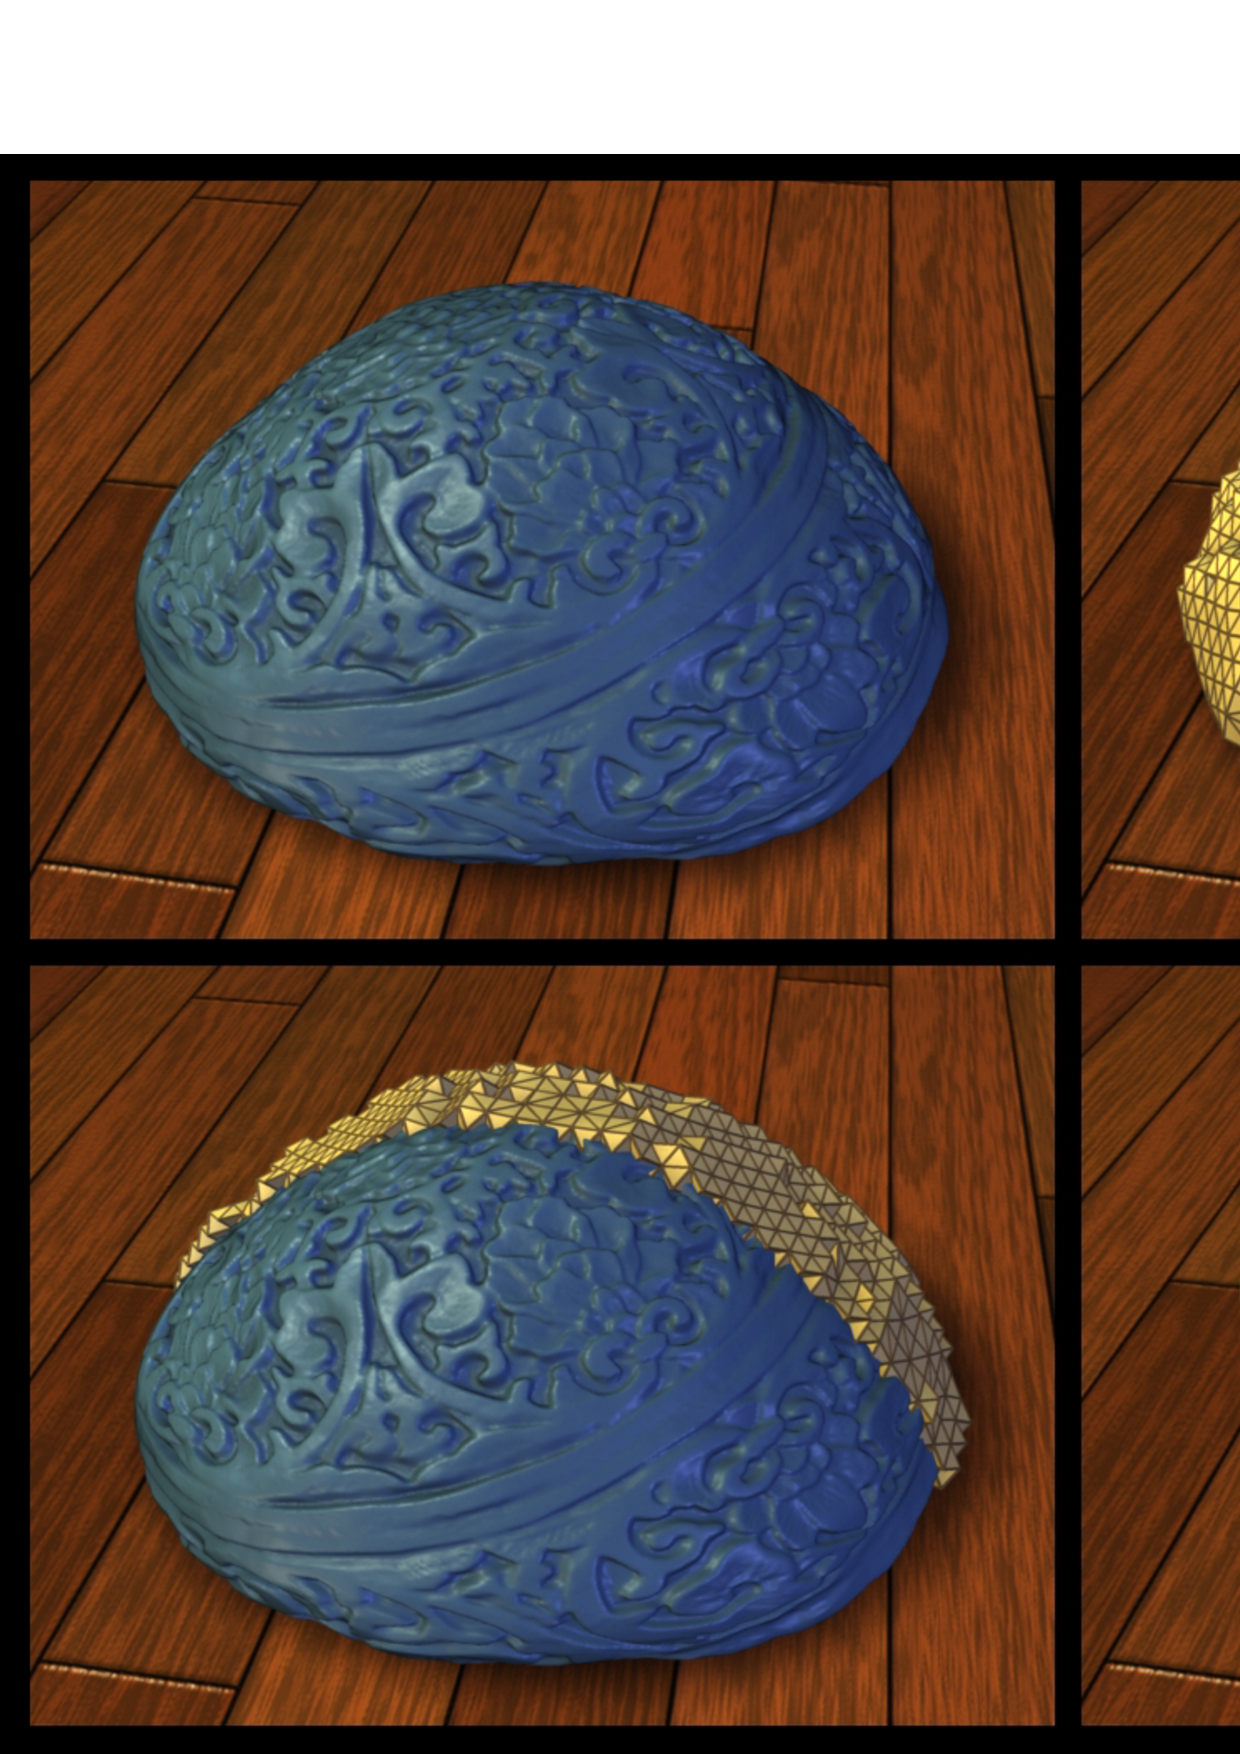
\includegraphics[width=0.8\linewidth]{images/starAdaptivity-cgf2016/WT2008_BCC.png}
	\caption[STAR adaptivity: Body-centered cubic mesh]{A high resolution surface mesh (blue) embedded into a deforming low resolution spatially-adaptive tetrahedral mesh based on a BCC lattice (gold). The bottom row shows the cross section of the tetrahedral mesh, illustrating the BCC structure. Image from Wojtan and Turk \cite{Wojtan2008}.}
	\label{fig:WT_BCC}
\end{figure}
Batty et al. \cite{Batty2010} use a similar meshing strategy to simulate inviscid fluids using a finite-volume discretization. The method also handles embedded solid and free-surface boundary conditions, even though the tetrahedral mesh does not conform to the domain boundaries. Batty and Houston \cite{Batty2011} extend this work by adding an implicit viscosity model. As explained later in the Section \ref{sec:meshless}, Ando et al. \cite{Ando2013} also use an adaptive BCC mesh for simulating liquids. Sifakis et al. \cite{Sifakis2007:Hybrid} introduce the concept of ``hard bindings'' to create an adaptive BCC lattice with T-junctions for the purposes of elastic solid simulation.
\\
Adaptively-refined BCC lattice is exceptionally useful in simulations requiring tetrahedral meshes, because the structured lattice makes the typically expensive operations of remeshing and re-sampling simulation data relatively insignificant. Although the structure of the mesh removes some control over the shapes and nature of the spatial adaptivity, the structure also eliminates typical issues, such as degenerate tetrahedra.

\paragraph*{Tall cell grids} Simulations of deep water also benefit from adaptive ``tall cell'' techniques~\cite{Irving2006,Chentanez2011}, which use regular grid cells near the water surface (where detail and accuracy is important), and tall rectangular fluid cells farther below the surface. This strategy effectively assumes that the behavior in regions located deep underwater is simpler, in that the simulation variables cannot change arbitrarily with depth. While we specifically discuss tall cell grids here because of their use of geometric adaptivity, we will also address some related height-field methods in Section \ref{sec:mixed-models}. These methods seem to work very well when the assumptions of the methods hold. However, there is reason to believe that artifacts (like spurious reflecting waves or dissipating vortices) can occur when the tall cells fail to properly resolve important dynamics.

\paragraph*{Far-field grid structures} Zhu et al. \cite{Zhu2013} propose a method for fluid simulation that maintains an efficient Cartesian grid structure but allows non-uniform spacing between the nodes.
This approach makes it easy to concentrate smaller cells where the domain is more interesting and retain larger cells farther away from areas of interest.
In addition to concentrating detail in important regions, this method also approximates non-reflecting boundary conditions by greatly extending the boundaries of the simulation domain.

\subsubsection{Unstructured meshes}
\label{sec:meshes}
Adaptivity on unstructured meshes is closely related to the problem of remeshing.
Considered purely as a geometrical problem, remeshing has been studied extensively in computational geometry \cite{Cheng2012} and in a modeling context in computer graphics \cite{Alliez2008}.
Indeed, the techniques adopted for adaptive simulation often build on the framework of geometrical remeshing methods, and extend them to a simulation context.
A number of challenges arise when performing remeshing during simulation, though.
First, the mesh elements must remain well-conditioned to avoid degrading the stability of the simulation.
Second, modifying the discretization on the fly risks introducing errors in transferring energy and momentum to the new mesh, such as numerical diffusion due to re-sampling, and discontinuous ``popping'' artifacts in thin strands or sheets.
Third, removing degrees of freedom must be done with care, as a mesh with fewer DOFs cannot represent the previous system state exactly.
Depending on the characteristics of the simulated material---whether it is elastic, plastic, or fluid; whether volumetric or lower-dimensional---different remeshing methods are found to be appropriate.
\begin{figure}[!ht]
	\centering
	\begin{subfigure}[b]{0.2\linewidth}
		\centering
		\includegraphics[width=\linewidth,valign=m]{images/starAdaptivity-cgf2016/remeshing-sqrt3.png}
		\caption{\label{fig:remeshing-sqrt3}}
	\end{subfigure}
	\hfill
	\begin{subfigure}[b]{0.2\linewidth}
		\centering
		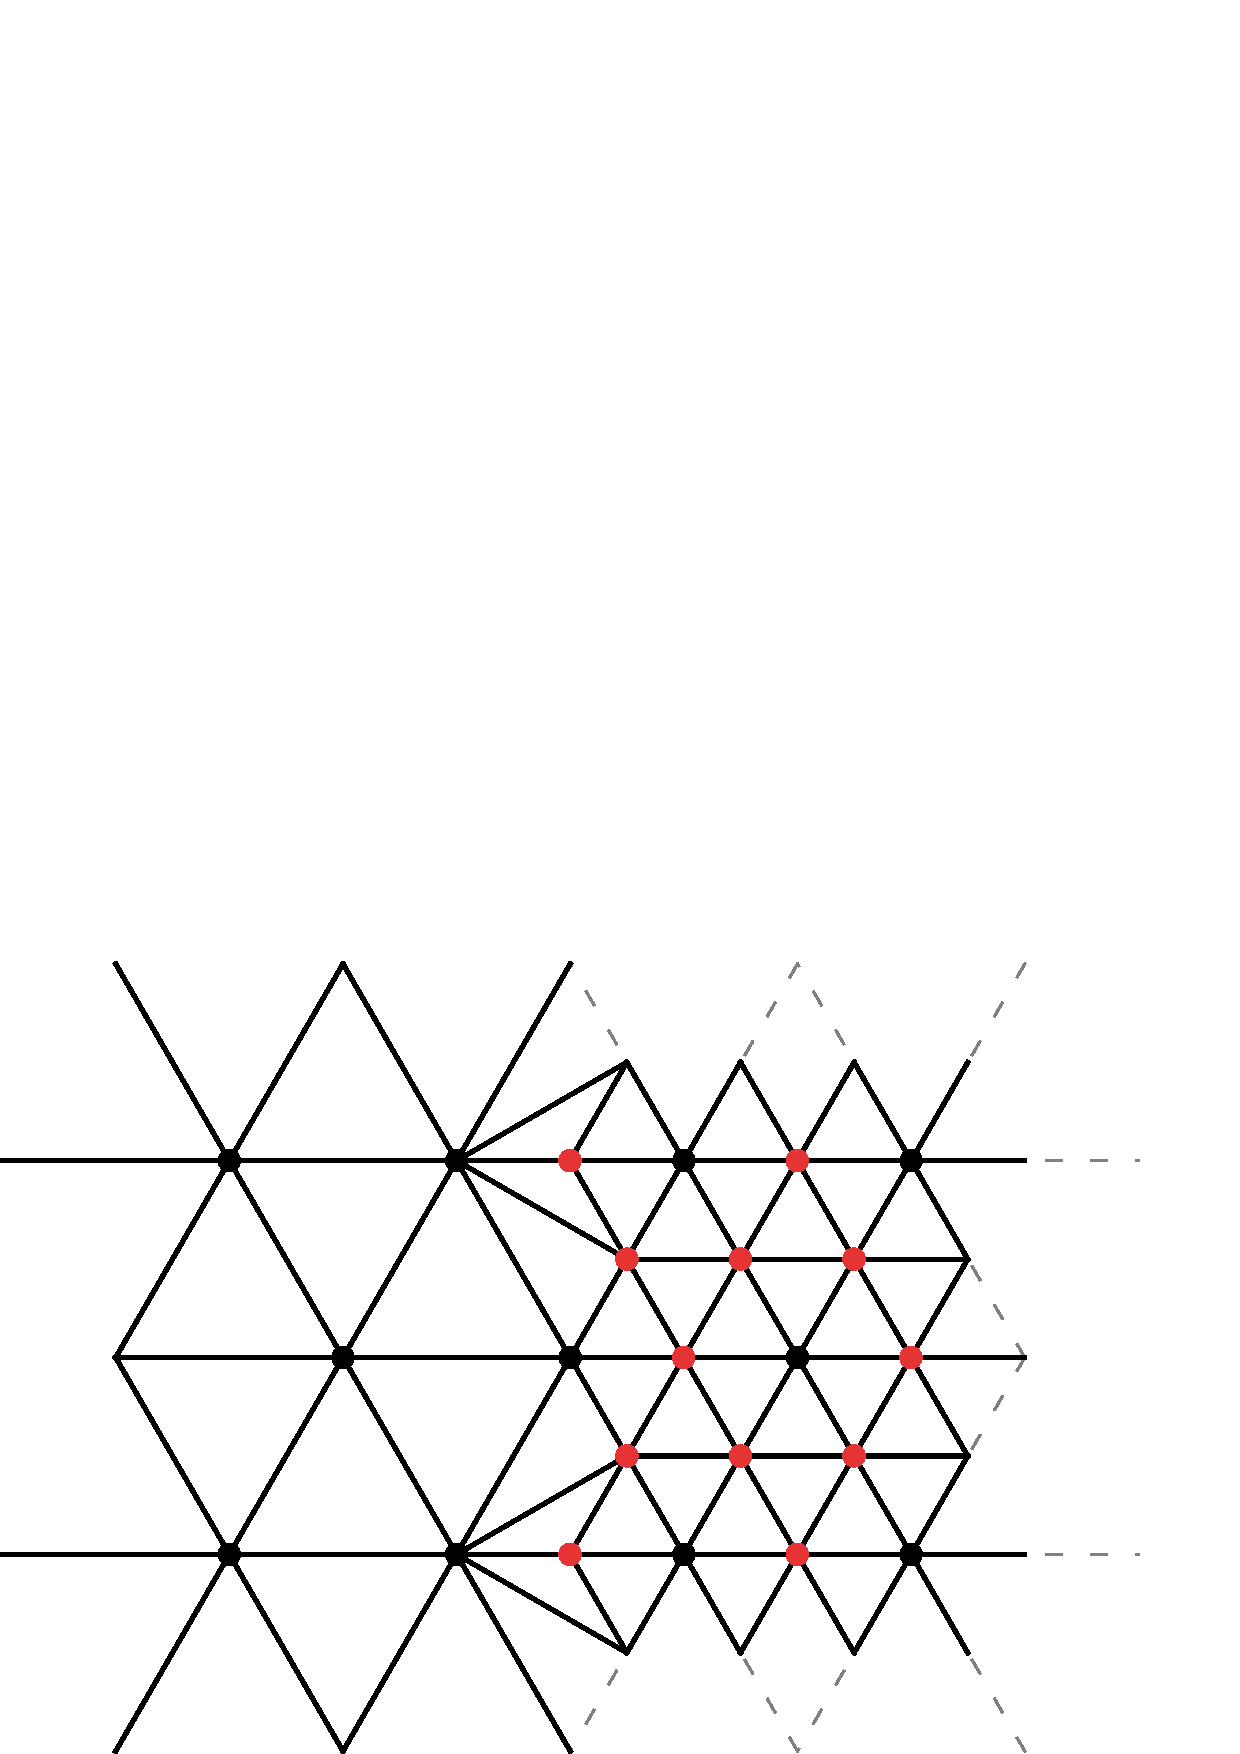
\includegraphics[width=\linewidth,valign=m]{images/starAdaptivity-cgf2016/remeshing-bisect.png}
		\caption{\label{fig:remeshing-bisect}}
	\end{subfigure}
	\hfill
	\begin{subfigure}[b]{0.2\linewidth}
		\centering
		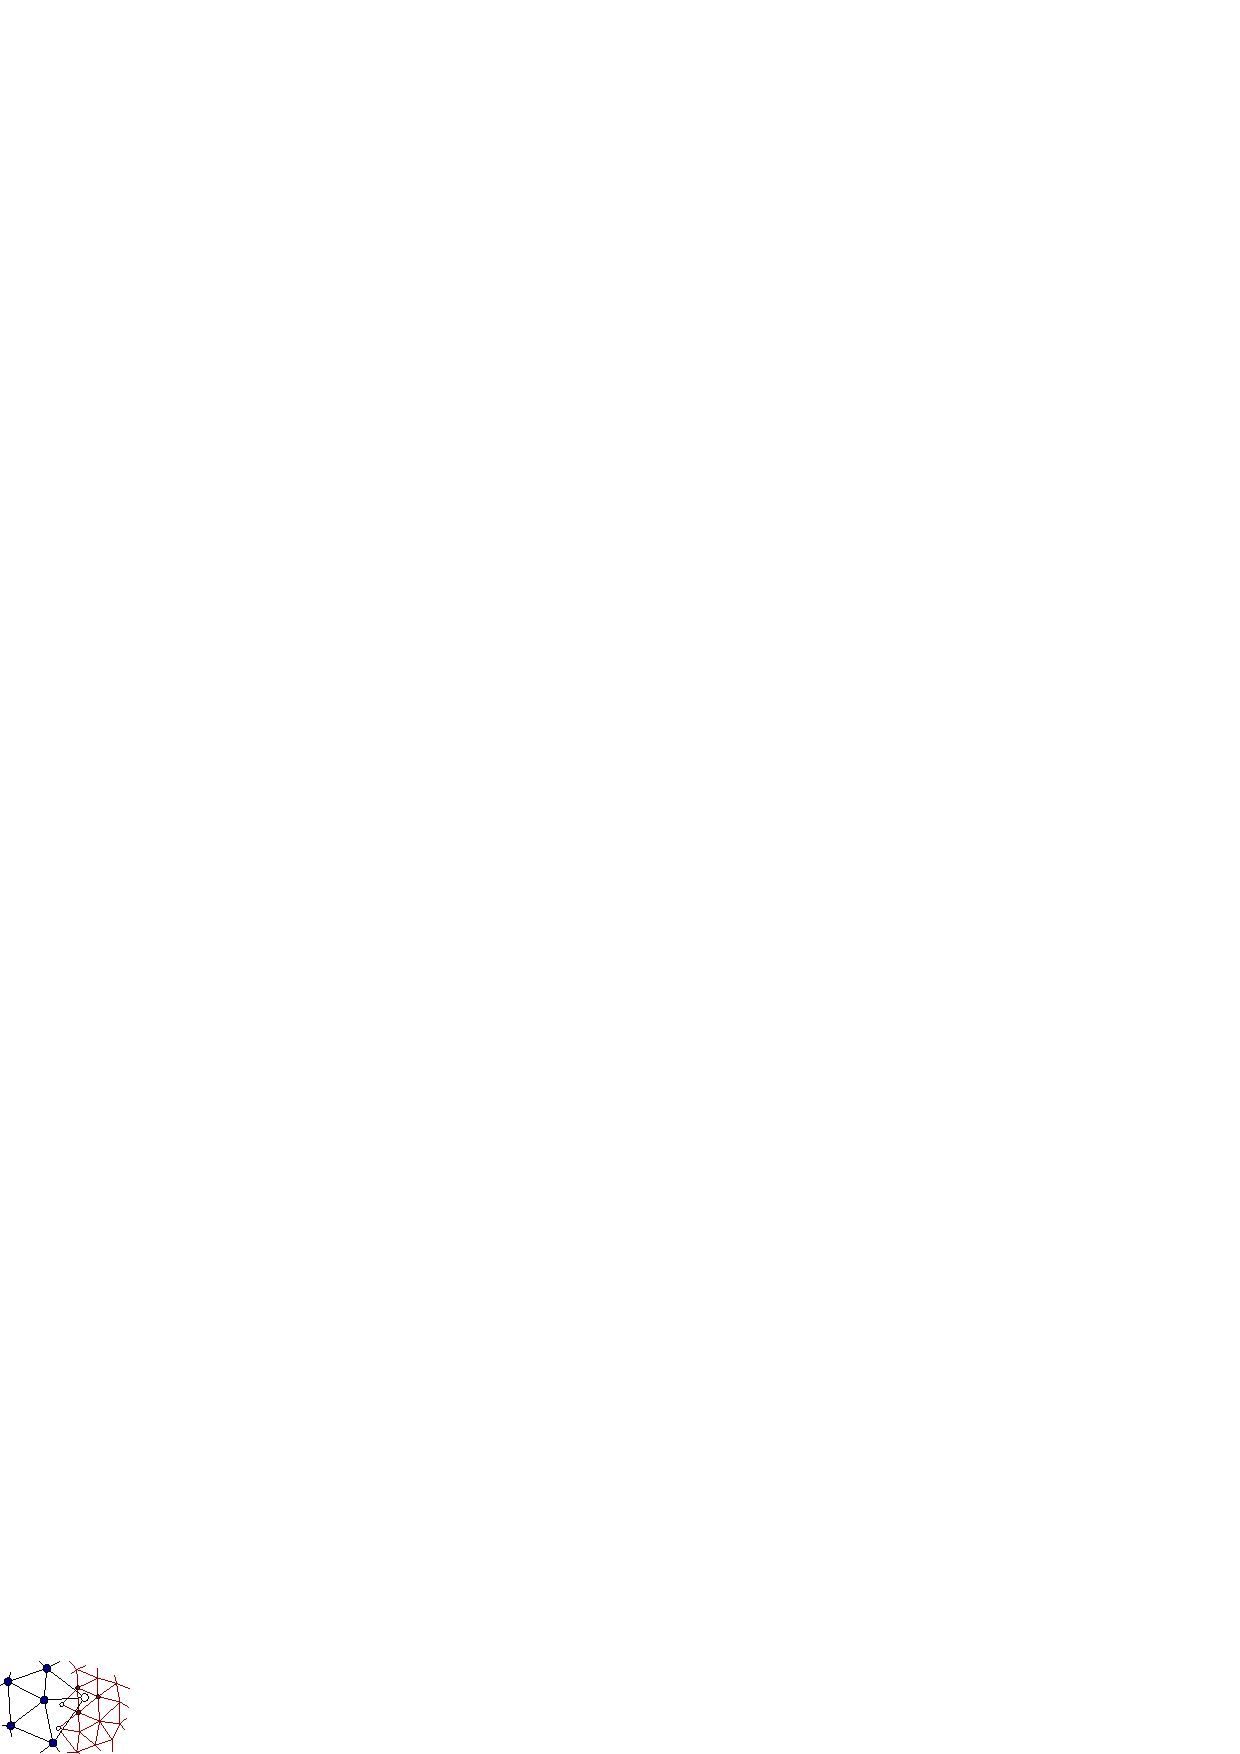
\includegraphics[width=\linewidth,valign=m]{images/starAdaptivity-cgf2016/remeshing-nonnested.png}
		\caption{\label{fig:remeshing-nonnested}}
	\end{subfigure}
	\hfill
	\begin{subfigure}[b]{0.3\linewidth}
		\centering
		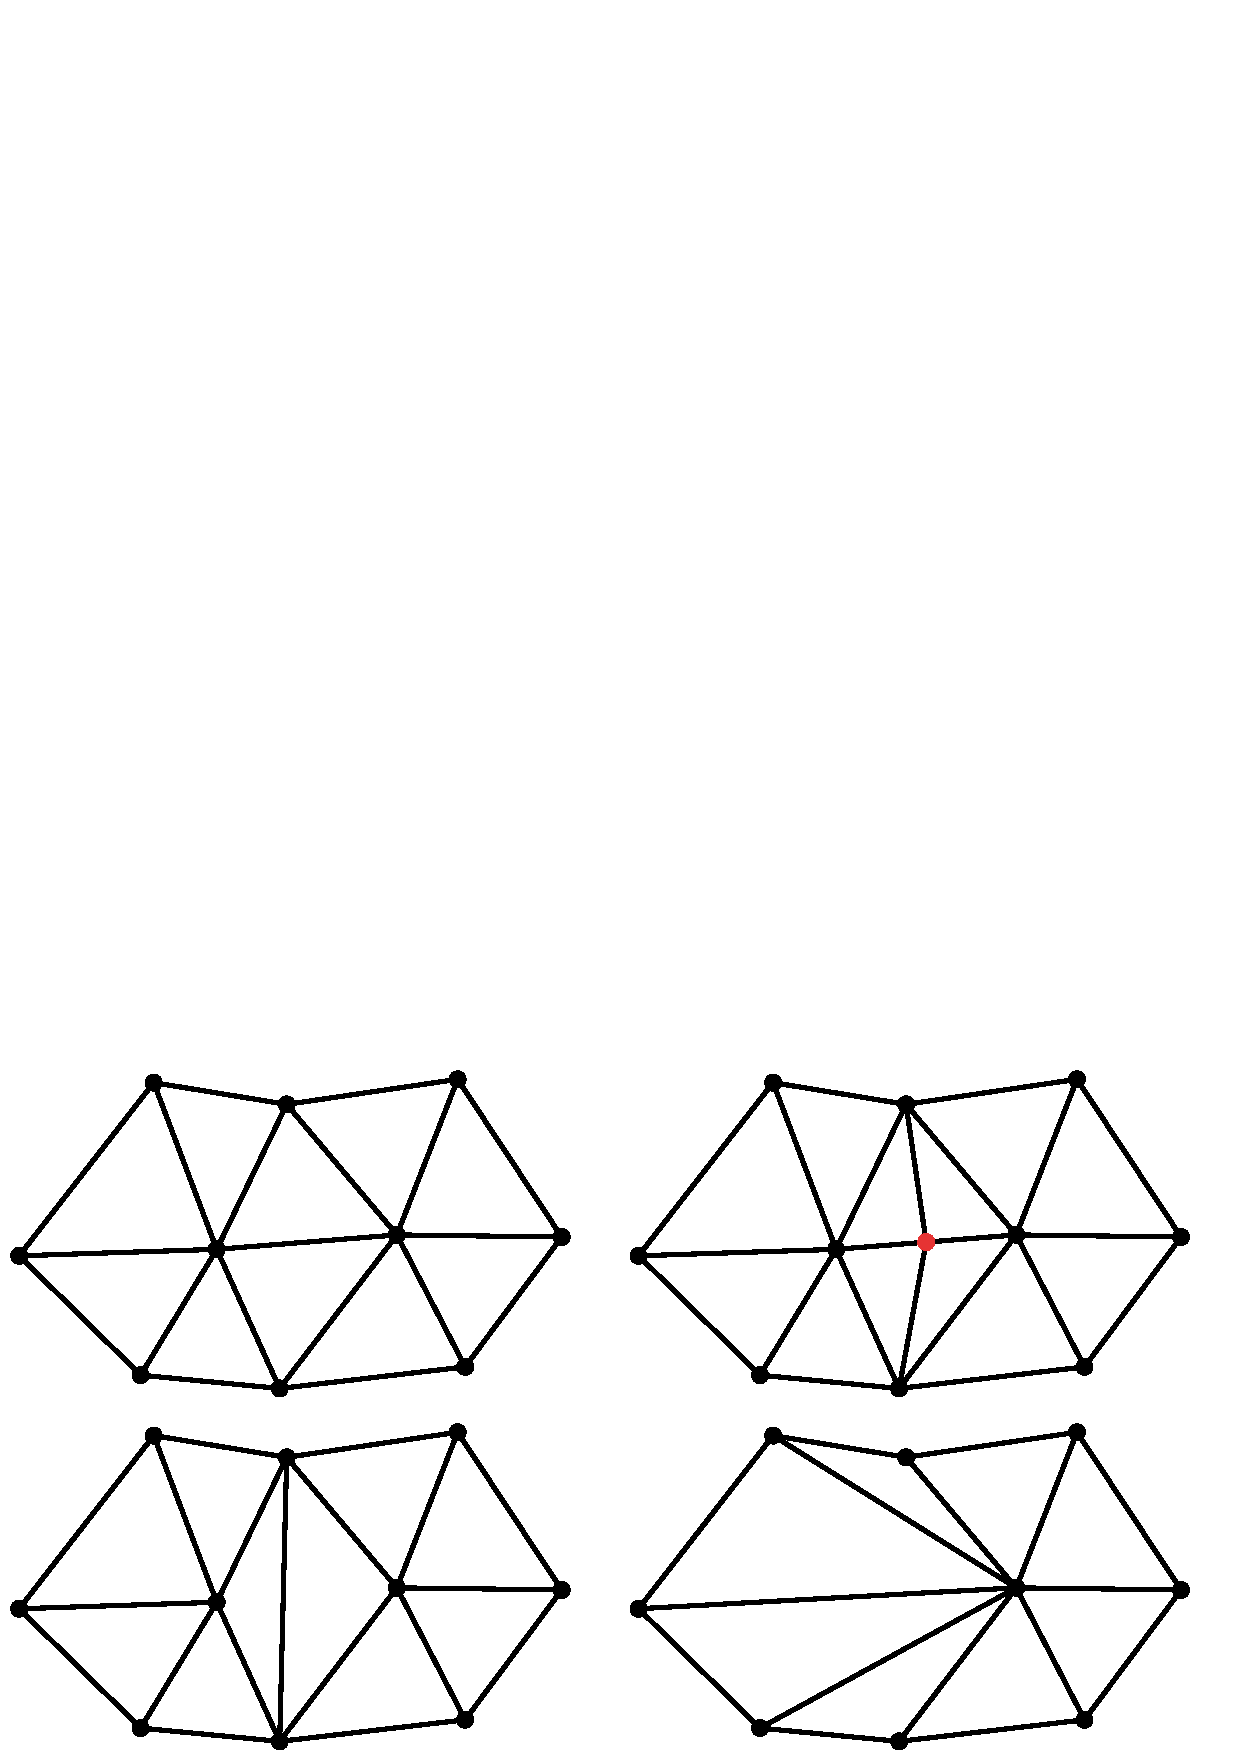
\includegraphics[width=\linewidth]{images/starAdaptivity-cgf2016/remeshing-local.png}
		\caption{\label{fig:remeshing-local}}
	\end{subfigure}
	\caption[STAR adaptivity: Refinement schemes for unstructured meshes]{   \label{fig:remeshing-schemes}
		Overview of refinement schemes for unstructured meshes. In (a) and (b), the right half of a mesh is refined using (a) $\sqrt3$ refinement and (b) hierarchical edge bisection, with inserted nodes highlighted in red. In (c), we illustrate two levels of non-nested meshes. In (d), the three primitive operations of local remeshing are applied to the middle edge: in reading order, we show the original mesh, after an edge split, after an edge flip, and after one of two possible edge collapses.}
\end{figure}
\paragraph*{Hierarchical schemes} The simplest remeshing strategy is to use a fixed hierarchical scheme for refinement, which provides guaranteed bounds on element quality.
Two such schemes are illustrated in Figure \ref{fig:remeshing-sqrt3}, \ref{fig:remeshing-bisect}.
In cloth simulation, triangle subdivision schemes such as 1-to-4 splits, $\sqrt3$ refinement, and edge bisection have been employed \cite{Li2005,Simnett2009,Bender2012:adaptiveFEM}.
A similar scheme for subdivision of tetrahedra was used by Koschier et al. \cite{Koschier2014} for volumetric fracture.
Wu et al. \cite{Wu2001} build on the concept of progressive meshes \cite{Hoppe1996} to precompute FEM parameters, allowing adaptive simulation of deformable bodies at interactive rates.
\\
However, subdivision schemes still degrade element quality by a moderate extent compared to an optimized mesh.
When this is undesirable, an alternative is to use a hierarchy of ``non-nested meshes'' at different resolutions \cite{Debunne2000,Debunne2001}; see Figure \ref{fig:remeshing-nonnested}.
Each level of the hierarchy is a complete mesh that does not necessarily share any nodes with meshes at other levels, and can be independently optimized \textit{a priori}.
At run time, regions at different levels of detail use subsets of different meshes.
Coupling is achieved by allowing the regions to overlap slightly; nodes in the overlap region in each mesh are treated as inactive ``ghost'' nodes that are embedded in the containing element of the other mesh.
The work of Otaduy et al. \cite{Otaduy2007} seamlessly integrates such adaptive non-nested meshes with a multi-grid algorithm and an adaptivity-aware collision detection technique.
\\
Hair simulation can benefit from adaptivity, as the contact interactions between hair strands lead to the formation of emergent clusters.
Bertails et al. \cite{Bertails2003} introduce a hierarchical structure called an adaptive wisp tree (AWT), which represents hair clusters that can progressively split into smaller clusters from the base to the tip.
Refinement is performed by splitting a node if its size and acceleration are large, while coarsening is performed by merging sibling nodes if they have similar positions and velocities.

\paragraph*{Nearly regular meshes}
Some techniques for liquid simulation use a structured mesh in the interior of the volume, but allow irregularities at boundaries to better capture the dynamics of the free surface.
These techniques benefit from many of the advantages of structured meshes discussed in Section \ref{sec:structured}, while still retaining much of the flexibility of unstructured meshes, such as the ability to accurately match boundary conditions.
\\
In such methods, one typically maintains a high-resolution representation of the surface as a triangle mesh that is updated at each time step.
The surface is superimposed on a regular mesh structure such as an octree or a uniform grid, and elements near the surface are modified, or new elements inserted, to better conform to the surface.
In particular, Chentanez et al. \cite{Chentanez2007} use the isosurface stuffing algorithm \cite{Labelle2007} that generates an adaptive BCC lattice whose surface tetrahedra are warped and possibly subdivided to conform to the surface geometry.
Using an octree to construct the lattice allows for coarser resolution away from the free surface.
Brochu et al. \cite{Brochu2010} use a uniform background lattice and introduce additional pressure samples along both sides of the free surface to ensure that all surface features are resolved.
The pressure projection is then performed on a mesh consisting of the Voronoi cells of these sample points.

\paragraph*{Local remeshing}
In some contexts, it is desirable to allow the connectivity structure of the mesh to be modified freely during the course of the simulation.
Such a requirement arises when anisotropic elements are needed to resolve strongly directional features, or when the material exhibits both elastic properties and unbounded deformation, such as in plastic flow.
\\
While it is possible to perform global remeshing---that is, simply creating a new simulation mesh from scratch whenever needed \cite{Klingner2006,Bargteil2007}---this approach can lead to undesirable diffusion of stored physical quantities such as plasticity information.
An increasingly popular alternative is to remesh locally using a set of local operations that refine, coarsen, and reshape existing elements.
In local remeshing techniques, any elements in the mesh that do not satisfy the desired size and shape criteria are improved by careful application of these operations.
This process is repeated until all mesh elements are satisfactory.
\\
When performing remeshing, it is important to ensure that the mesh remains well-conditioned for simulation, through the use of various element quality measures \cite{Shewchuk2002}.
In 2D, the Delaunay triangulation optimizes several important notions of mesh quality, including the minimum angle and the maximum circumradius of any triangle, but the Delaunay tetrahedralization in 3D provides few such guarantees, and more sophisticated mesh improvement strategies may be required \cite{Wicke2010}.
If anisotropic remeshing is desired, the remeshing criterion is often expressed through a spatially varying metric tensor $\mathbf M$, with the goal being that each edge $\mathbf e$ should have $\mathbf e^T\mathbf M\mathbf e\approx1$.
Equivalently, we desire $\|\mathbf M^{1/2}\mathbf e\|\approx1$; that is, we want edges to be of unit length and elements to be equilateral in the transformed space of $\mathbf M^{1/2}$.
This viewpoint allows element quality metrics and Delaunay properties defined for isotropic meshes to be carried over to the anisotropic setting.
\\
For manifold triangle meshes, high-quality remeshing can be accomplished using only the three simple operations of edge split, edge collapse, and edge flip (see Figure \ref{fig:remeshing-local}).
Narain et al. \cite{Narain2012} use these operations in cloth simulation, generating an adaptive anisotropic mesh that resolves detailed wrinkles and folds (see Figure~\ref{fig:Narain2012}).
\begin{figure}[!h]
	\centering
	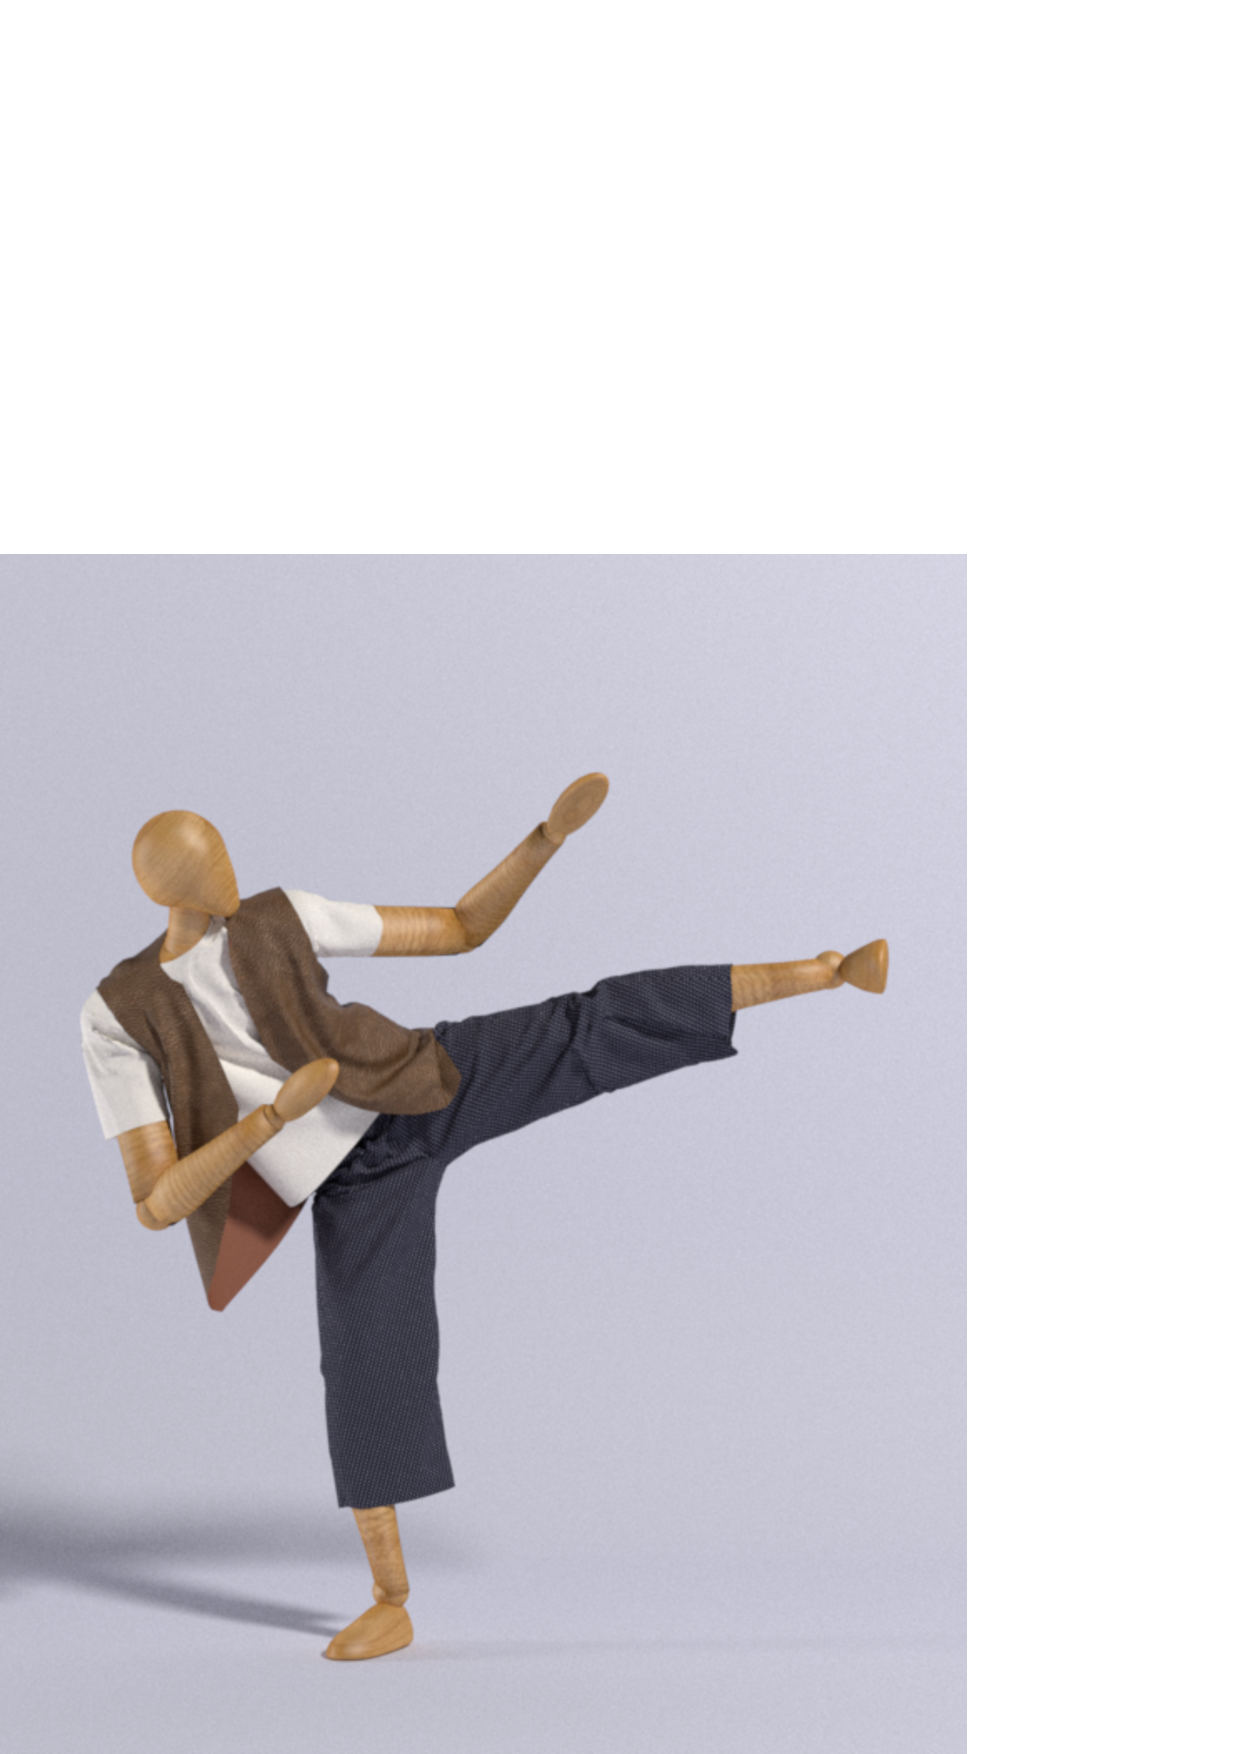
\includegraphics[width=0.35\linewidth]{images/starAdaptivity-cgf2016/cloth-render.png}
	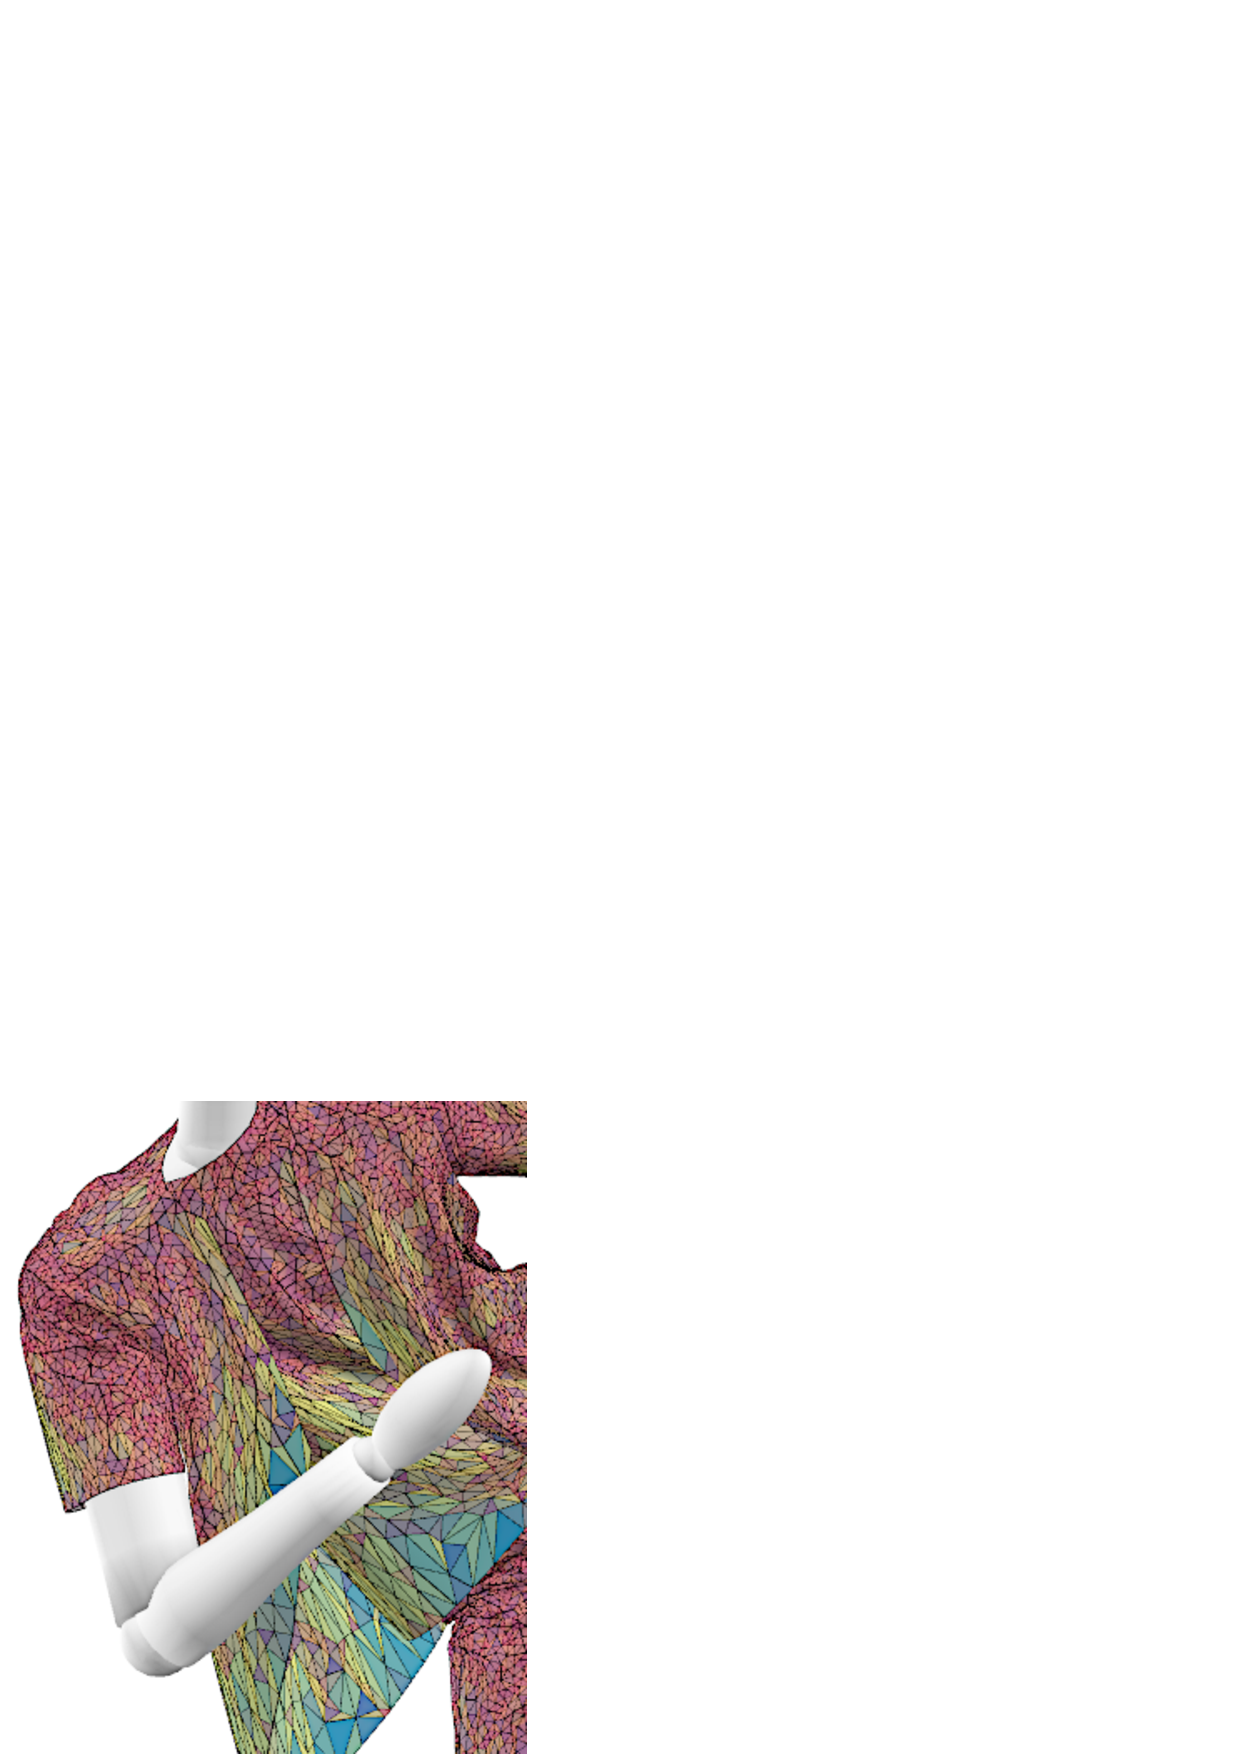
\includegraphics[width=0.35\linewidth]{images/starAdaptivity-cgf2016/cloth-wire-zoom.png}
	\caption[STAR adaptivity: Anisotropic remeshing of triangular meshes]{The anisotropic remeshing algorithm of Narain et al. \cite{Narain2012} allows detailed wrinkles in cloth to be resolved accurately with fine elements (red), while much coarser elements (blue/green) are used in flat regions. Long, narrow folds are best represented using anisotropic elements (yellow) aligned with the curvature direction.}
	\label{fig:Narain2012}
\end{figure}
First, all edges that are unacceptably long according to the refinement criterion are split, then edge collapses are attempted as long as they do not create new unacceptable edges.
During both steps, edge flips are performed to maintain an approximately Delaunay mesh relative to the anisotropic metric.
\\
Local remeshing of tetrahedral meshes is significantly more involved, requiring several different local operations and a complex schedule for the order in which to apply them \cite{Klingner2007}.
This technique was first applied to simulation by Wicke et al. \cite{Wicke2010}, who used it to minimize artificial diffusion in elastoplastic flow.
Subsequent work has applied such remeshing techniques to simulation of incompressible liquids \cite{Misztal2012a,Misztal2012b,Clausen2013}.
\\
Misztal et al. \cite{Misztal2012a,Misztal2012b} build a mesh over the entire simulation domain, with some elements belonging to the fluid and the rest to the exterior, while Clausen et al. \cite{Clausen2013} mesh only the fluid volume.
The former approach allows topological changes like collisions to be handled automatically without special treatment, although at the cost of maintaining a mesh over a potentially much larger domain.
Clausen et al. also describe techniques for guaranteeing incompressibility and momentum conservation that are applicable to both approaches. 
Two key advantages offered by these methods are that (i) the advection step causes no numerical diffusion, because physical quantities move with the mesh nodes, and that (ii) surface tension can be modeled accurately thanks to an explicit surface representation tied directly to the simulation mesh.
\\
Apart from simply adding or removing vertices, surface tracking algorithms in fluid dynamics may also move vertices along the surface in order to optimize mesh shapes.
A process called ``null-space smoothing'', which slides vertices within the tangent space of a meshed surface, is used in several works \cite{Jiao2007,Brochu2009,Brochu2010,Wicke2010,Clausen2013}.
This strategy improves the quality of simulation elements without changing the shape of the tracked surface.

\paragraph*{Additional challenges and techniques}

When refinement is performed, the position of the newly inserted node has to be chosen carefully.
Simply placing it at the midpoint of the original element can cause physical quantities such as bending to change discontinuously, injecting artificial energy into the system and leading to instabilities.
Instead, it is better to adjust the mesh locally to bring it into an energy-minimizing configuration.
Spillmann and Teschner \cite{Spillmann2008} consider the positions of the new node $\mathbf x_i$ and its neighbors as variables and perform an optimization to minimize the total energy,
\begin{equation}
	U(\mathbf x_1,\ldots,\mathbf x_n) - \sum_{j=1}^n\mathbf f_j^T\mathbf x_j,
\end{equation}
where $U$ is the internal energy due to elastic forces, and $\mathbf f_j$ is the external force acting on node $j$.
A similar approach has been used for simulating the behavior of stiff two-dimensional sheets such as paper and metal \cite{Narain2013,Pfaff2014}, but with $\mathbf f_j$ replaced with an acceleration-corrected term $\mathbf f_j - m_j\mathbf a_j$ to preserve the instantaneous acceleration of each node.
\\
Liquids with surface tension may freely transition between volumes, thin films, filaments, and droplets; representing these transitions is a challenge for most mesh-based techniques.
Zhu et al. \cite{Zhu2014} address this problem using non-manifold meshes of mixed dimensionality, composed of tetrahedra, triangles, segments, and points.
Beyond the traditional remeshing operations that work within a single dimensionality, they also provide operations for dimensionality transitions via element collapse (e.g. transforming a thin triangle to a segment) and merging (e.g. generating a tetrahedron to connect two adjacent triangles with small dihedral angle).
\\
Finally, we point out the recent ``power particles'' technique of de Goes et al.~\cite{deGoes2015}, which builds an unstructured mesh at each time step using a Voronoi-style power diagram.
This can be viewed as a global remeshing approach like the ones mentioned above \cite{Klingner2006,Bargteil2007}, but this method stores physical quantities on Lagrangian particles without maintaining an explicit connectivity, and thus avoids numerical diffusion due to re-sampling.
While this work is not specifically an adaptive strategy, it is a form of spatial discretization that makes adaptivity very easy to implement, and could be a fruitful basis for future work in adaptive simulation.

\subsubsection{Meshless models}
\label{sec:meshless}
In the last two decades, numerous meshless models have been extended to perform adaptive physically-based animation. They include Smoothed-Particle Hydrodynamics (SPH) (see the survey of Ihmsen et al. \cite{Ihmsen2014:STAR}), fluid-implicit particle (FLIP) (see the seminal work of Zhu and Bridson \cite{Zhu2005}), moving least squares (MLS) (see Muller et al. \cite{Muller2004:melting}) and frame-based models (see Gilles et al. \cite{Gilles2011}). These models were used to describe a wide range of phenomena, from fluids (SPH, FLIP) to solids (MLS, frame-based).
\\
Due to the absence of fixed connectivity, meshless models are among the most flexible models for spatial adaptivity. This flexibility, combined with the variety of models, leads to an impressive number of re-sampling strategies, developed to resolve details near splashes, large deformations, viscoplastic flows and fractures. We classify these strategies into three categories: (1) dynamic local re-sampling, (2) multi-scale methods, and (3) hierarchical refinement (see Figure \ref{fig:particleOverview}).
\begin{figure}[t]
	\centering
	\begin{subfigure}[b]{0.20\linewidth}
		\centering
		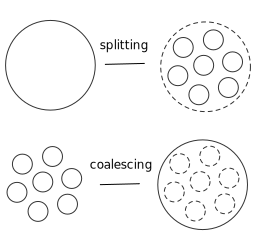
\includegraphics[width=\linewidth]{images/starAdaptivity-cgf2016/particles-operators.png}
		\caption{\label{fig:meshless-operators}}
	\end{subfigure}
	\hfill
	\begin{subfigure}[b]{0.45\linewidth}
		\centering
		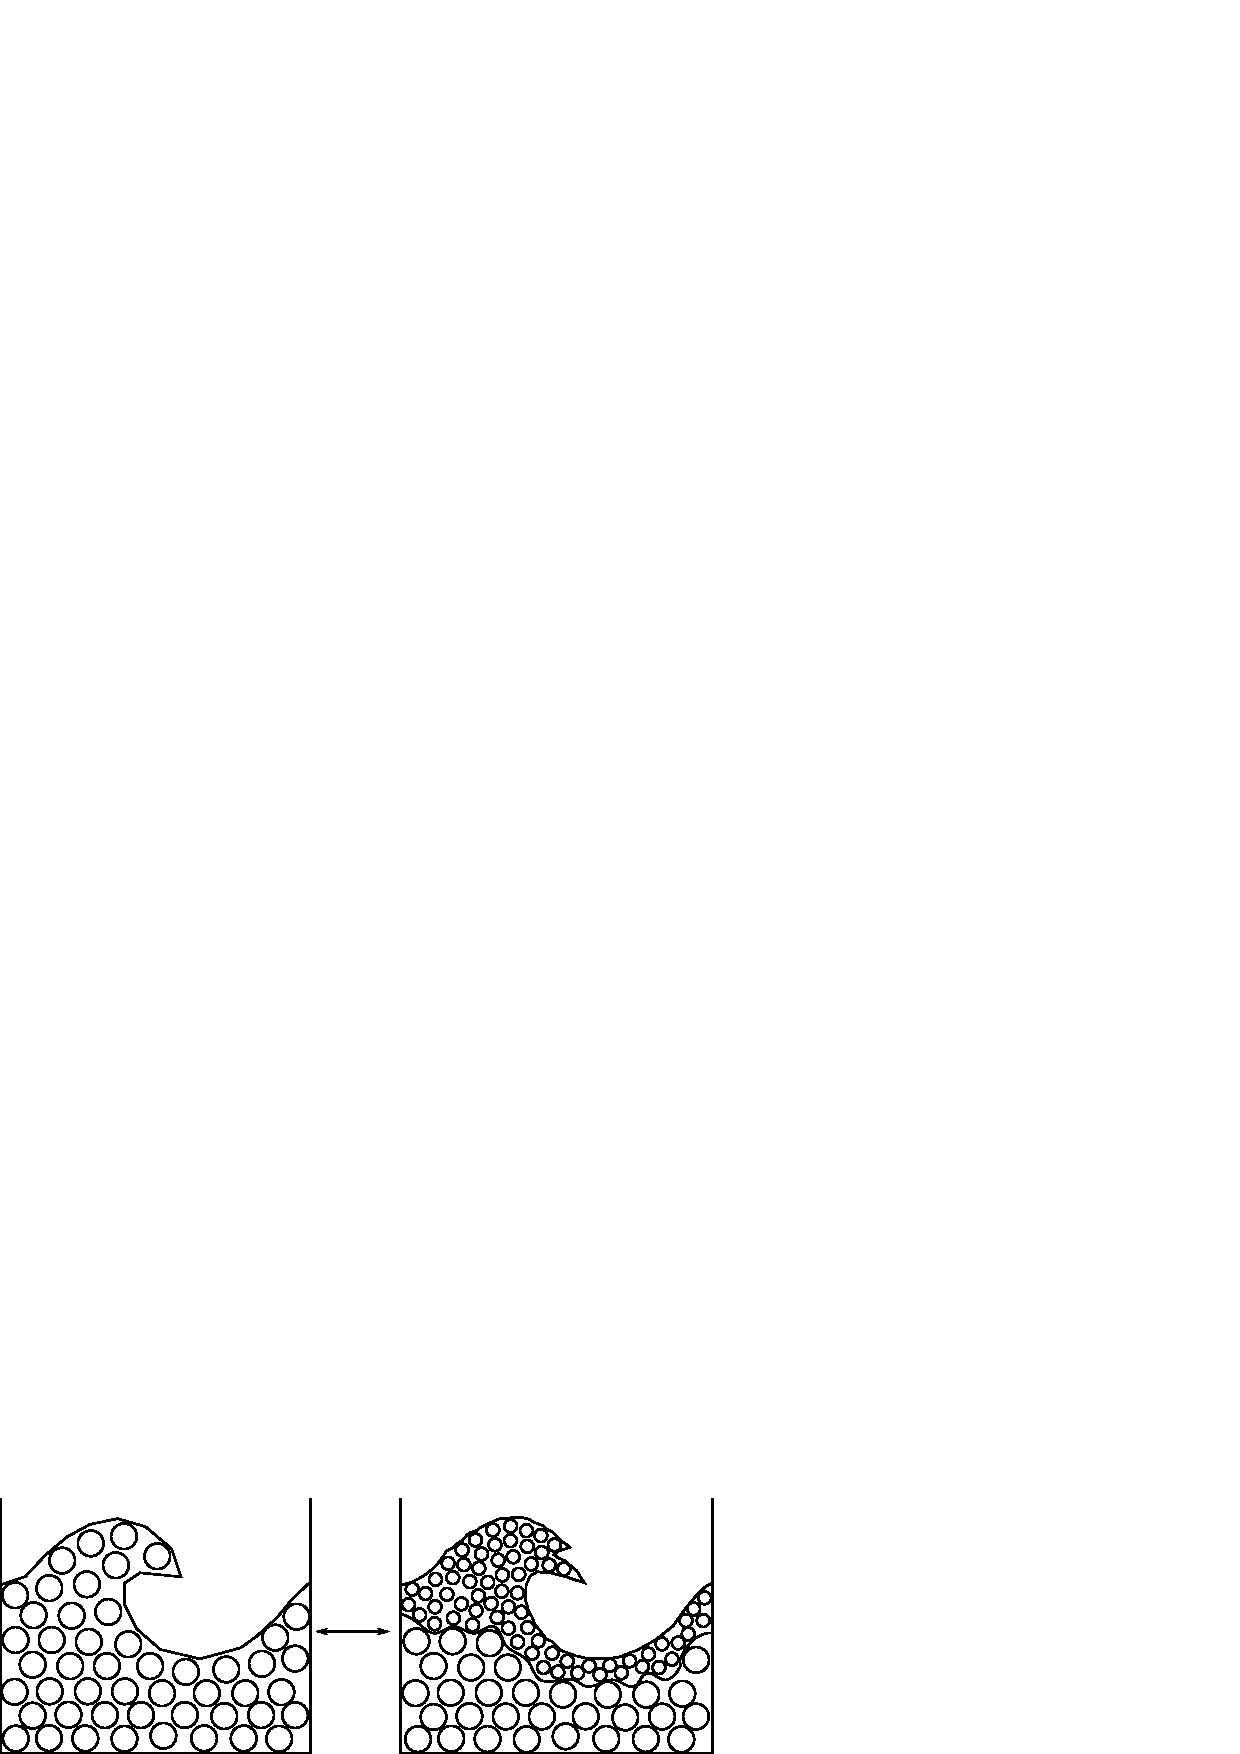
\includegraphics[width=\linewidth]{images/starAdaptivity-cgf2016/particles-multiscale.png}
		\caption{\label{fig:meshless-multi-scale}}
	\end{subfigure}
	\hfill
	\begin{subfigure}[b]{0.3\linewidth}
		\centering
		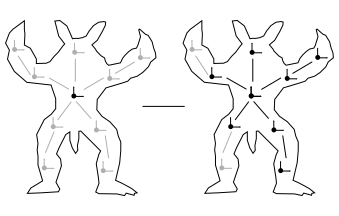
\includegraphics[width=\linewidth]{images/starAdaptivity-cgf2016/particles-hierarchy.png}
		\caption{\label{fig:meshless-hierarchy}}
	\end{subfigure}
	\caption[STAR adaptivity: Meshless techniques]{\label{fig:particleOverview}
		Overview of adaptive meshless techniques.
		(a) Dynamic local re-sampling applies splitting and coalescing operators to degrees of freedom in order to locally refine and coarsen regions of interests (b) Multi-scale methods couple several simulations with different resolutions. Coarser simulations are used as boundary conditions for the finer resolutions. Feedbacks from the finer resolutions are used to avoid divergences between two different resolutions. (c) Hierarchical refinement dynamically activates or deactivates levels of a precomputed hierarchy between degrees of freedom.}
\end{figure}
\\
These different strategies make meshless models particularly useful for material that undergo large irreversible deformations such as the one cited above. However, it is important to keep in mind that the flexibility of meshless models come with expensive nearest-neighbor search algorithms to determine the connectivity between material samples at run time.
\\
We inform the reader that complementary information about SPH adaptive techniques can be found in the state-of-the-art report by Ihmsen et al. \cite{Ihmsen2014:STAR}.

\paragraph*{Dynamic local re-sampling} The idea is to dynamically subdivide or merge particles to fit a desired resolution (see Figure \ref{fig:meshless-operators}). The success of this strategy mainly relies on the re-sampling scheme's ability to ensure stability, to accurately represent boundaries, and to prevent popping artifacts. Depending on the underlying model (SPH, FLIP, MLS) and its sensitivity to intense re-sampling, different strategies have been proposed.
\\ \\
As a full particle-based method, the SPH model is a perfect candidate to dynamic re-sampling. Yet, its sensitivity to particle distribution makes re-sampling strategies challenging. First, the interaction between particles with different sizes increases the error in the pressure term, leading to instabilities. Therefore smooth grading of resolution is required to minimize this error. Second, the change of positions during re-sampling can create a sudden change in density which will result in violent pressure forces, which again lead to instabilities (see Orthmann and Kolb \cite{Orthmann2012}).
Several methods that can be combined were proposed to avoid these local change in density. First, instead of computing the density based on positions, one can use the continuity equation as done by Desbrun and Cani \cite{Desbrun1999}. In order to avoid integration error to be accumulated along the simulation, the density still needs to be re-computed based on positions at a user-defined interval. Then, one can perform position optimization to minimize errors during re-sampling \cite{Adams2007} and use quantity blending over time to smooth out inevitable sampling error \cite{Orthmann2012}.
Also, it is important to keep in mind that another challenge is to efficiently retain the parallel nature of SPH in the adaptive scheme. Zhang et al. \cite{Zhang2008} and Yan et al. \cite{Yan2009} propose two different methods to make splitting and merging operators parallel.
\\ \\
More recently, dynamic re-sampling has been applied to FLIP. As FLIP is a combination of grid and particles, two levels of adaptivity are possible: one on the grid resolution, and the other on the particle sampling. Also, only advection operations are performed on the particles, which results in a less position-sensitive simulation and allows much more flexibility than SPH. More precisely, FLIP does not apply density-based forces to the particles. Consequently, sudden density changes due to particle splitting or merging do not have the same catastrophic consequences as in SPH. However, damping is introduced once particles are merged. This can be taken into account by changing blending parameters of the FLIP simulator as suggested by Ando et al. \cite{Ando2012}.
Early works on adaptive FLIP perform adaptivity only on particles based on a deformability criterion and the distance to surface \cite{Hong2008FLIP, Ando2012}. Ando et al. use the flexibility of FLIP regarding the particles' positions in order to preserve fluid sheets by creating additional particles.
In both methods, the largest particle size is bounded by the cell size of the underlying grid, which precludes aggressive adaptive sampling and the use of a fully adaptive FLIP simulator. Ando et al. \cite{Ando2013} combine an adaptive BCC mesh (see Section \ref{sec:structured}) with adaptive particle sampling to handle highly different resolutions. (see Figure \ref{fig:Ando2013}).
\begin{figure}[t]
	\centering
	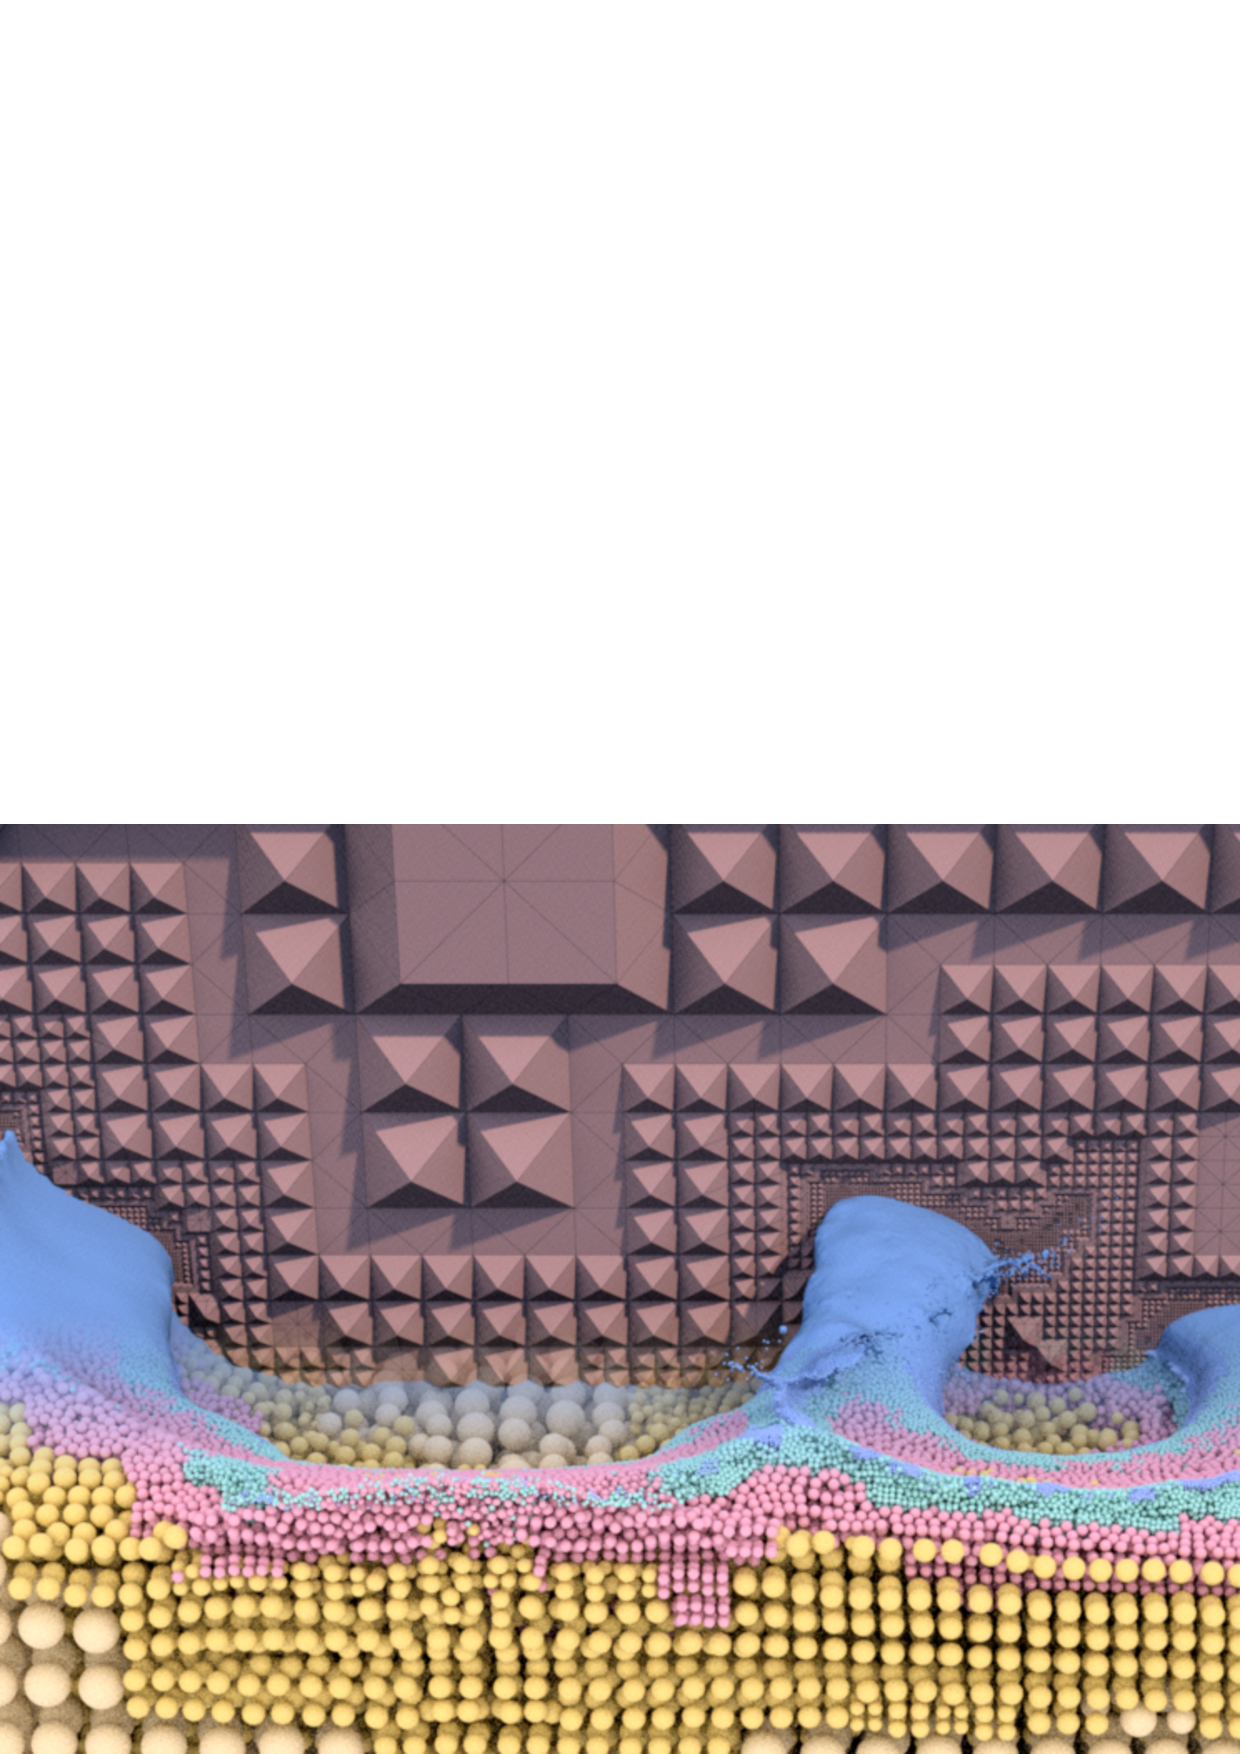
\includegraphics[width=0.8\linewidth]{images/starAdaptivity-cgf2016/Ando2013_3.png}
	\caption[STAR adaptivity: Hybrid refinement of meshes and particles]{Ando et al. \cite{Ando2013} simulate liquid by combining adaptively-sized FLIP particles (bottom, front) with an adaptive tetrahedral mesh for the pressure solve (top, back).}
	\label{fig:Ando2013}
\end{figure}
\\ \\
When simulating solids, local re-sampling is essential in describing phenomena such as large deformations and fracture. First, like mesh-based methods, large deformations create poorly sampled regions leading to ill-conditioned deformation gradients and instabilities. Second, as explained in Section \ref{sec:spatial_refinement}, a challenge in fracture simulation is to reach a sufficiently fine discretization near the tip of the crack in order to obtain a realistic crack path. In these cases, local re-sampling can greatly improve accuracy and stability while retaining efficiency. However, there are two main challenges that require special care.
\\
The first one consists in accurately describing material discontinuities. Most of the time, shape functions are spherical and they must be modified so that sharp boundaries can be represented. In their work on large viscoplastic deformation and fracture, Pauly et al. \cite{Pauly2005} model discontinuities using extended shape functions with transparency criteria, and locally modify a sparse neighborhood graph to update connectivity. Another strategy was proposed by Steinemann et al. \cite{Steinemann2009} to address the high cost of shape functions update. It consists in using a visibility graph to efficiently handle connectivity and approximate material distances used in computing shape functions.
\\
The second one comes from rendering artifacts that can occur at the surface due to splitting. In this context, Jones et al. \cite{Jones:2014:DEF} propose a strategy to re-sample elastoplastic simulation while alleviating popping artifacts. They base their method on the evaluation of each particle neighbor's density. This evaluation is performed using a weighted covariance matrix computed in rest space for each particle $i$, where $\mathbf{u}_{ij}$ denotes the vector between particle $i$ and particle $j$, its neighbor.
\begin{equation}
\label{eq:jones_re-sampling}
\mathbf{B}_{i} = \sum_{j}  \frac{\mathbf{u}_{ij}\mathbf{u}_{ij}^{T}}{\| \mathbf{u}_{ij} \|^{4}}
\end{equation}
If the maximum eigenvalue of $\mathbf{B}_{i}$ is too small, then there are too few particles in the neighborhood and the particle is split in two. New particles are positioned along each side of the eigenvector with the minimum eigenvalue. In order to prevent from rendering artifacts, splittings which are not tangent to the surface are rejected, and particles near the surface are split along the middle eigenvector whose direction is tangent to the surface. Conversely, if the minimum eigenvalue of $\mathbf{B}_{i}$ is too large, then there are too many particles in the neighborhood and the particle is merged with its closest neighbor. The new particle is positioned halfway between the two merged particles.

\paragraph*{Multi-scale methods}
In multi-scale methods, several simulations with different resolutions are coupled in a hierarchical way (see Figure \ref{fig:meshless-multi-scale}).
At the coarsest simulation level $L_{0}$, the whole domain is discretized. Then, each finer simulation level $L_{r}$ discretizes a subset of $L_{r-1}$ with a finer scale. This finer subset is defined to match regions of interests that can be physically or visually motivated. Transitions between two scales are bilateral: the coarsest simulation level $L_{r}$ is used to build boundary conditions for the finer simulation level $L_{r+1}$ and feedbacks from a finer simulation level $L_{r+1}$ to a coarser simulation level $L{r}$ are applied, in order to prevent dynamics of two different levels from diverging. Solenthaler and Gross \cite{Solenthaler2011} and Horvath and Solenthaler \cite{Horvath2013} apply this idea to SPH fluid simulation.
Compared to merging and splitting particles, the main advantage is that interactions between different resolutions are not direct anymore. Thus, stability can be more easily ensured and large differences in resolution can be handled.
In Solenthaler and Gross's approach, a two-scale simulation is performed. High-resolution regions are defined based on the distance to the surface and the view frustum. In these regions, low-resolution particles emit finer particles according to a cubic pattern which ensures a uniform space sampling. Relaxation steps are performed when particles enter the high-resolution region in order to avoid large pressure forces. Horvath and Solenthaler extend the two-scale simulation to multi-scale simulation, and avoid previous artifacts such as mass loss due to particle removal and instabilities due to oversampling near boundaries.

\paragraph*{Hierarchical refinement}
Dynamic re-sampling techniques were also used in frame-based methods to simulate elastic deformations, see \cite{Gilles2011} for a full description of the method. Tournier et al. \cite{Tournier2014} use a hierarchical approach to achieve simplifications during deformation without popping artifacts (see Figure \ref{fig:meshless-hierarchy}). The material is deformed using physically-based control frames organized in a generalized hierarchy. The model can be simplified by attaching frames to their parents at any time in their current relative positions. Activation and deactivation of nodes is performed based on relative velocity and user-specified metrics, while integration points are updated according to the hierarchy. These hierarchical techniques take advantage of their structure to improve efficiency, but may lack of flexibility, especially regarding topological changes.

\subsection{Miscellaneous techniques for spatial adaptivity} \label{sec pr adaptivity}

By far the most popular approach to spatial adaptivity in computer graphics is to add more computational elements where more accuracy or detail is desired, as surveyed in Section \ref{sec:spatial_refinement}. This type of spatial adaptivity is often called \textit{h}-refinement, because the length of an edge in a mesh is typically indicated by the letter $h$. In addition to this tried-and-true strategy, there are other fundamentally different approaches for achieving spatial adaptivity. In the next sections, we will discuss strategies that refine the basis within a single element (a superset of \textit{p}-refinement, which refers specifically to the order of a polynomial basis) and during a subspace simulation, strategies that use multiple grids that move and overlap to track locations where more detail is desired, and strategies that mix different reference frames in order to use the computational degrees of freedom optimally.

\subsubsection{Basis refinement}
\label{sec:basis_refinement}
If we wish to achieve spatial adaptivity without explicitly remeshing (perhaps because it is difficult to control element quality when remeshing, or because a particular application requires that we preserve the original mesh), then we can perform basis refinement instead. The concept of basis refinement can be a difficult one to grasp for newcomers to the field. One of the best ways to understand basis refinement is in the context of finite element methods (FEM). In generic terms, FEM attempts to approximate a function (typically the solution to a partial differential equation) with a very limited, very specific subset of all possible functions. Most methods in computer graphics use linear interpolation within each element, which essentially restricts the solution to a piecewise linear function. For the purposes of this discussion, we would say that the elements are using linear basis functions, and that the overall solution is expressed in a piecewise-linear basis. However, we can actually represent the solution more accurately (in the sense that the solution converges more quickly under refinement) by using more elaborate bases, like piecewise quadratic functions instead of piecewise linear ones.

This section discusses four types of basis refinement: hierarchical basis refinement, polynomial basis refinement, basis enrichment, and adaptive reduced basis functions.
The first three topics discuss adaptivity at the level of basis functions, whereas the fourth is about the adaptive creation of reduced basis in reduced model simulations.

\paragraph*{Hierarchical basis refinement}
In computer graphics, hierarchical basis refinement has mainly been applied to finite element simulations (FEM) of solids and shells \cite{Capell2002,Grinspun2002}. The idea is to refine computational basis functions instead of elements. From a theoretical point of view, there are no differences between hierarchical basis refinement and hierarchical element refinement. Both adaptively add more degrees of freedom with increasingly local support in order to improve accuracy where needed. Both use hierarchical schemes in order to efficiently sample the simulation domain.
The main differences are practical. By refining basis functions instead of elements, compatibility between regions with different resolutions are implicitly handled.
This makes adaptivity much easier and general.
\\
For instance, hierarchical basis refinement allows a simple handling of \emph{T-junctions}.
In FEM, each element's node carries a basis and builds a local stiffness matrix from its node's stiffness which are then assemble into a global stiffness matrix.
During this process, only independent degrees of freedom should add their contribution to the global matrix. However, when using hierarchical element refinement, non-independent degrees of freedom are added during the subdivision of the simulation mesh. They are called \emph{T-junctions} or \emph{T-nodes} (see Figure \ref{fig:tjunctions}) and require specific handling. Suddenly, a simple subdivision scheme becomes dependent on the dimensionality, the element type and the basis order, thus requiring important implementation work. In contrast, hierarchical basis refinement handles \emph{T-nodes} at the basis level by making sure that no bases are redundant. The hierarchical structure makes this process simple and thus offers a more general framework for adaptivity which can handle arbitrary resolution differences.
\begin{figure}[!h]
	\centering
	\begin{tabular}{cc}
		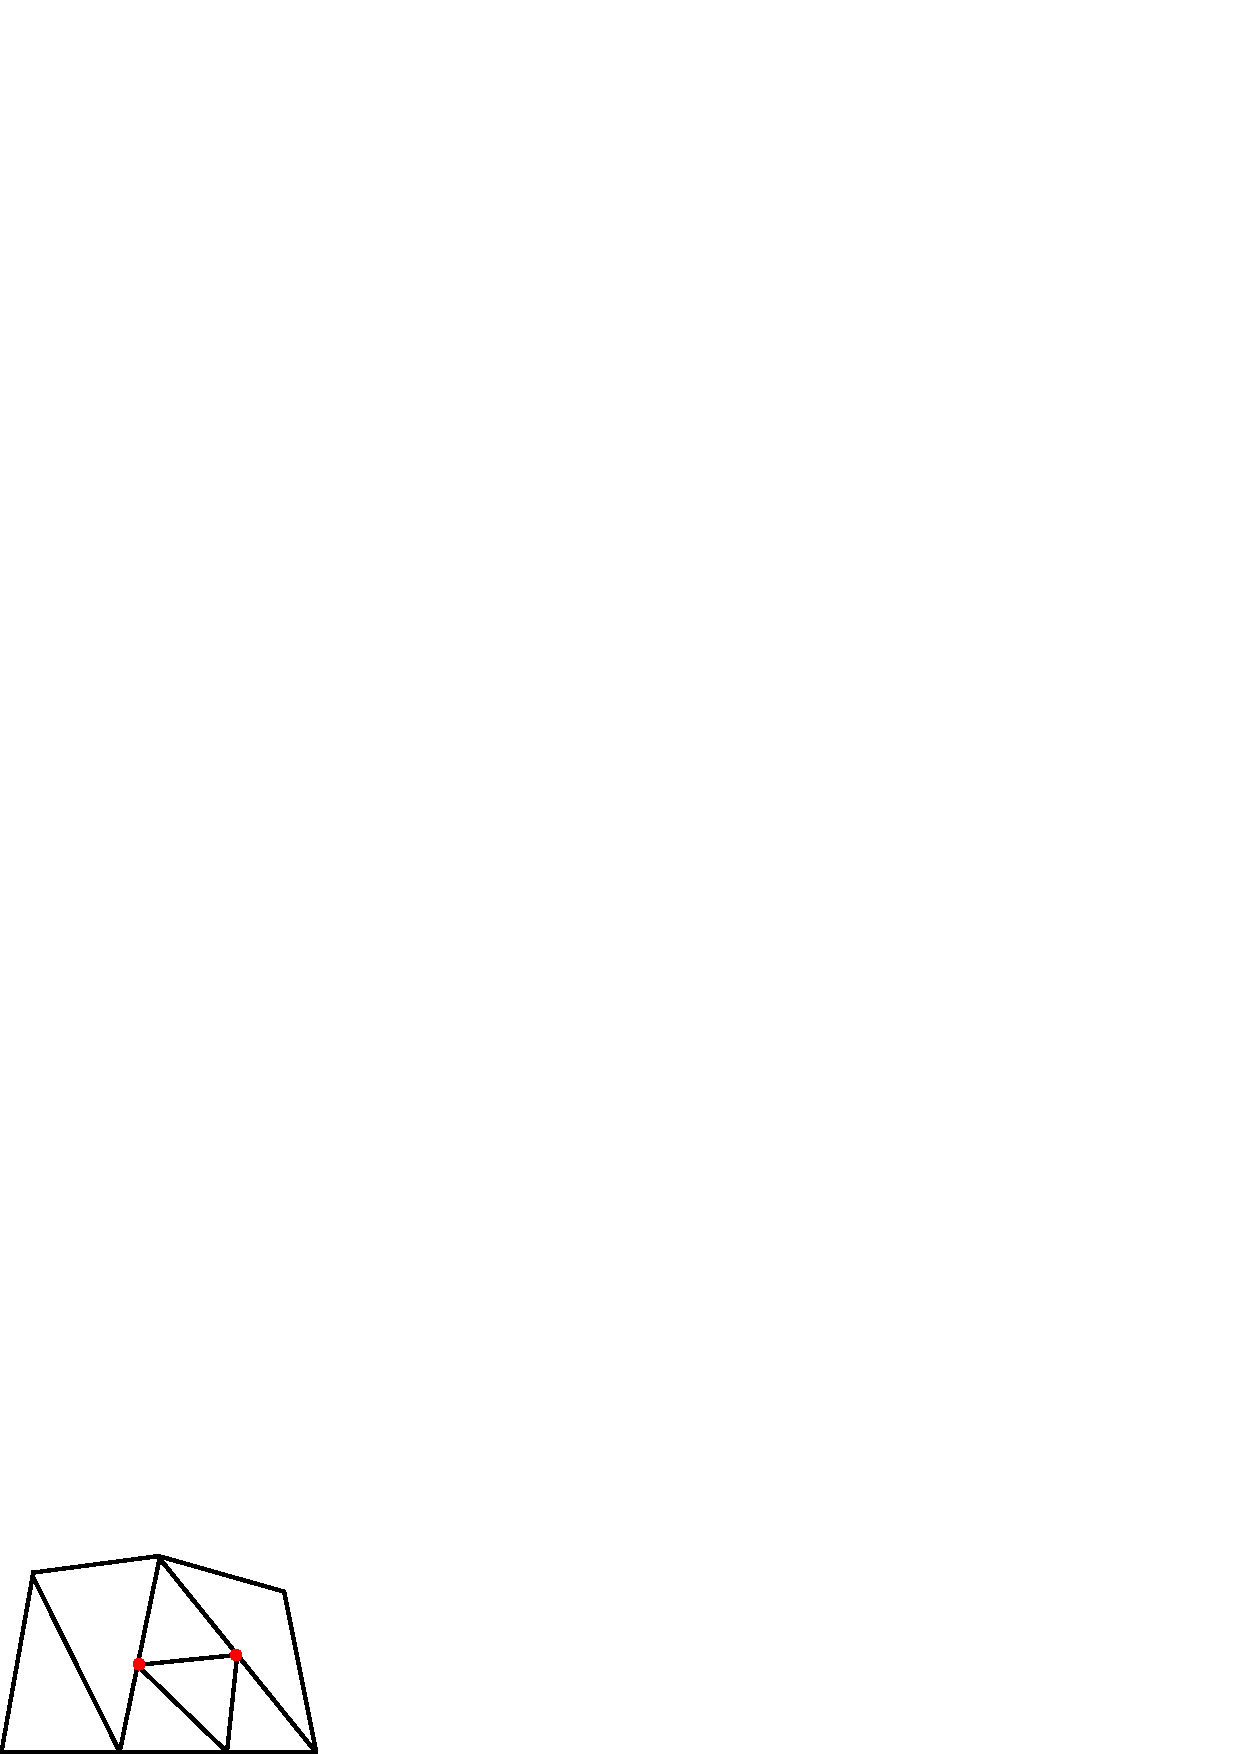
\includegraphics[width=0.35\linewidth]{images/starAdaptivity-cgf2016/tjunction-triangle.png} &
		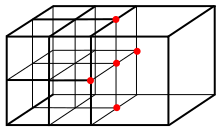
\includegraphics[width=0.35\linewidth]{images/starAdaptivity-cgf2016/tjunction-grid.png} \\
		(a) & (b)
	\end{tabular}
	\caption[STAR adaptivity: T-junction]{\label{fig:tjunctions} Refinement by element subdivision is attractive by its simplicity for 2D and 3D meshes, however it introduces T-junctions (in red) at interface between resolutions with different sizes. Bookkeeping or extra-remeshing operations are required to take care of these non-independent degrees of freedom.}
\end{figure}
\\
Capell et al. \cite{Capell2002} embed a high-resolution mesh in a hexahedral complex and precompute a hierarchy of bases up to a given level of refinement. During the simulation, depending on the amount of deformation, each level of the hierarchy will refine or coarsen, thus updating the current set of active bases. Basically, it is the same idea of \cite{Debunne2001} but from a basis point of view.
\\
The Conforming Hierarchical Adaptive Refinement Methods (CHARMS) framework of Grinspun et al. \cite{Grinspun2002} generalizes the idea of spatially refining the bases instead of the elements. They provide an in-depth explanation of the concept and describe numerous results of basis refinement applied to shells, solids and electrocardiography simulations.
In fact, it is quite surprising that this method was not more studied or extended in the last decade. A possible explanation is the fact that, in the last few years, adaptivity proved to be essential for large and complex deformations such as visco-elastic, visco-plastic flows. In those cases, hierarchical refinement is not sufficient anymore to ensure well-conditioning of the system matrices. 

\paragraph*{Polynomial basis refinement}
Polynomial basis refinement methods, also called \emph{p-adaptivity}, increase or decrease the order of the basis functions.
For a given spatial resolution, this allows to improve the quality of the deformation without remeshing. In computer graphics, using high order approximation to resolve fine details is not new. However mixing different orders of approximation to adaptively resolve details was only recently applied in the context of fluid simulation and elastic deformations.
\\
For fluid simulation, the smoothness of velocity and pressure makes \emph{p-adaptivity} potentially much more efficient than geometric adaptivity, because the error per degree of freedom decreases exponentially with the approximation order but only geometrically with the spatial resolution. In this favorable context, Edwards and Bridson \cite{Edwards2012,Edwards2014} use polynomial basis refinement in a Discontinuous Galerkin FEM framework in order to simulate detailed water with coarse grids. They use low-order bases deep inside the liquid and increase the basis order closer to the liquid surface, where more visual detail is desired (see Figure \ref{fig:pfluid}). By using basis refinement instead of element refinement, they can keep the simple structure of a low resolution Cartesian grid while pushing back the limit on the scale of details in one cell. In terms of cost, their method is approximately as expensive as a classical high spatial resolution simulation but it provides much more details such as extremely thin sheets.
\begin{figure}[t]
	\centering
	\begin{subfigure}[!ht]{0.48\linewidth}
		\centering
		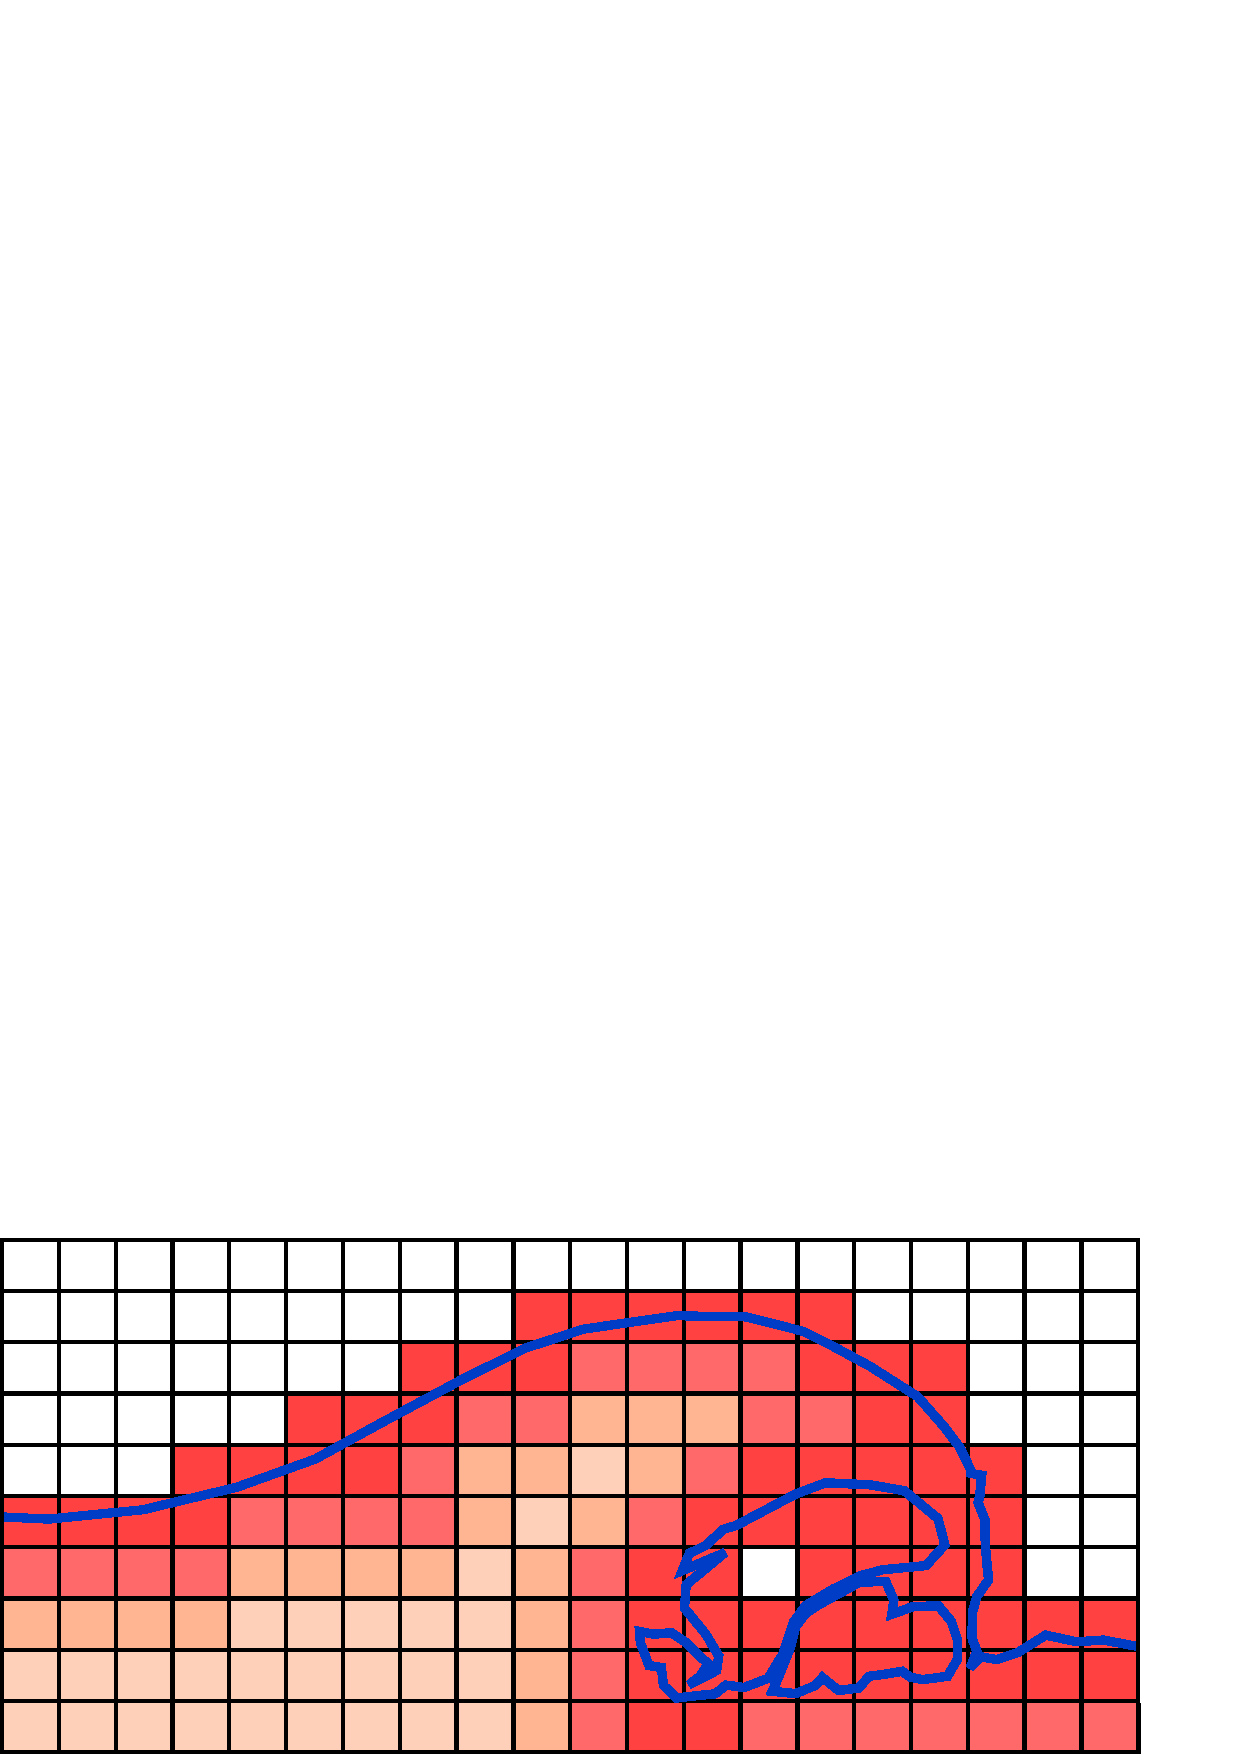
\includegraphics[width=\linewidth]{images/starAdaptivity-cgf2016/pfluid.png}
		\caption{\label{fig:pfluid}}
	\end{subfigure}
	\hfill
	\begin{subfigure}[!ht]{0.48\linewidth}
		\centering
		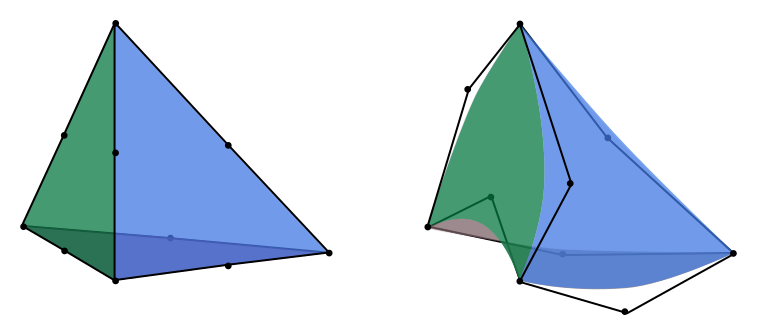
\includegraphics[width=\linewidth]{images/starAdaptivity-cgf2016/quadratic.png}
		\caption{\label{fig:quadratic_fem}}
	\end{subfigure}
	\caption[STAR adaptivity: p-adaptive techniques]{\label{fig:padaptivity}
		Illustrations of p-adaptive techniques for (a) fluids and (b) deformable solids.
		In (a) Each fluid cell uses a different approximation space depending on its distance to surface (blue line). Surface cells (in red) use fourth order polynomial to precisely approximate pressure. A smooth grading of the approximation is performed inside the fluid (lighter cells) that allows to save computational time.
		In (b) the canonical tetrahedron with quadratic control points and next to it the quadratic deformation induced by the deformed control mesh. Such a deformation would require many linear elements.
	}
\end{figure}
\\
Bargteil and Cohen \cite{bargteil2014animation} animate deformable bodies by combining linear and quadratic B{\'e}zier elements.
The main advantage of their method is the ability to locally increase degrees of freedom and to simulate nonlinear geometry without remeshing (see Figure \ref{fig:quadratic_fem}).
To decide whether an element should be linear or quadratic, they compare the linear and quadratic predicted positions of the midpoint of each edge of the element. If the difference between the two positions is larger than a threshold then the edge becomes quadratic. If the difference is less than another threshold then it becomes linear. Thus, some elements can have linear and quadratic edges, usually in transition regions. Bargteil and Cohen observe that, as the number of degrees of freedom increases, visual differences between linear and quadratic elements become difficult to discern. Moreover, the additional cost remains important and local deformations on the surface of a quadratic element due to collisions still cannot be resolved without element refinement. Therefore, their method is particularly efficient on low-resolution models, where it provides smoother geometry and better dynamics quality.
\\
In both cases, the differences of resolution between two regions that can be achieved only using \emph{p-adaptivity} are limited. An important avenue for research would be to combine those methods with geometric adaptive techniques. Such methods have been well studied in engineering fields and are called \emph{hp-adaptive} methods.

\paragraph*{Basis enrichment}

Another way to add spatial detail to a physical model without remeshing is by using ``basis enrichment.'' The main idea behind basis enrichment is to adaptively add carefully-chosen basis functions that are specifically designed for the phenomena being modeled. (This is in contrast to p-refinement, which is restricted to polynomial functions, regardless of the phenomena being simulated.) For an example of basis refinement, consider an object is being fractured; some material that used to be connected together will have to be split in two. A simple linear basis function could be split into two functions that are linear on one side of the fracture and zero on the other, as illustrated in Figure \ref{fig:basisenrichment}. 
\begin{figure}[t]
	\centering
	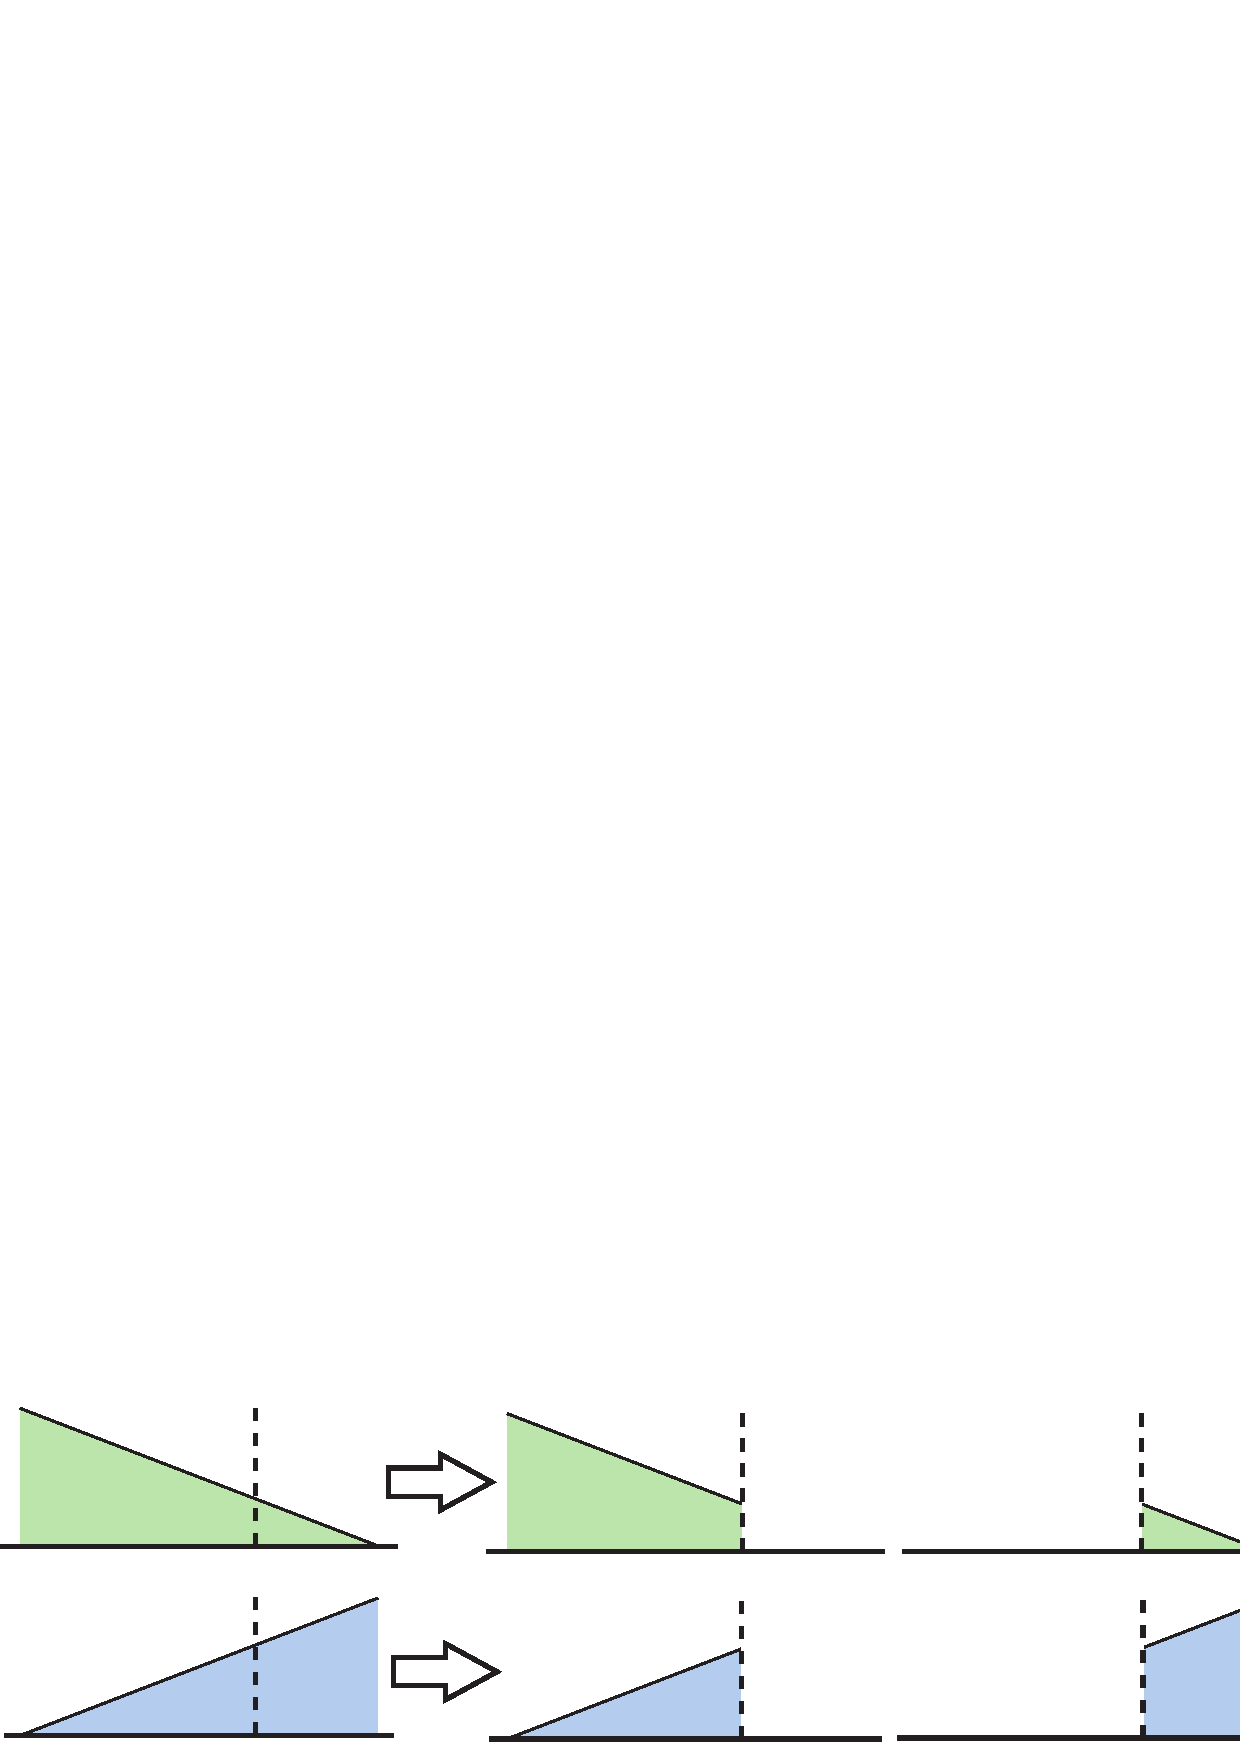
\includegraphics[width=0.8\linewidth]{images/starAdaptivity-cgf2016/xfem.png}
	\caption[STAR adaptivity: XFEM illustration]{\label{fig:basisenrichment}
		A one-dimensional element with linear basis functions can simulate a fracture by enriching its basis. Here, the new basis functions drop off to zero on the other side of the fracture site indicated by the dashed line, directly encoding the severed connection.
	}
\end{figure}
\\
This type of basis replacement effectively avoids remeshing by inserting a fracture directly into the basis itself. Note that in this case, we opted to enrich the basis with these particular ``step'' functions which drop to zero after a certain point, instead of trying to fit some polynomial that might overshoot or otherwise imperfectly capture the desired physics. Such basis enrichment techniques have been termed the ``general finite element method'' (GFEM) or ``extended finite element method'' (XFEM) \cite{belytschko2009review}.
\\
Adaptive basis enrichment methods have been recently applied in many computer graphics contexts.
The virtual node algorithm uses basis enrichment to stabilize fracture and cutting simulations~\cite{Molino2004,hegemann2013level}. Instead of remeshing and potentially inserting poorly-conditioned elements, the virtual node algorithm essentially copies the entire element and adapts its basis functions to the fracture site. The virtual node algorithm  has recently been improved to robustly allow multiple cuts in a single element \cite{Sifakis2007:Cutting,Wang2014}. One drawback to adaptive basis enrichment is that complicated cuts can require arbitrarily complicated basis functions that may not be simple to compute. In the case of cutting thin shells, Kaufmann and colleagues~\cite{Kaufmann2009} note that the most physically-appropriate enrichment functions require the solution of a Laplace equation with time-varying boundary conditions. Similar basis enrichment techniques may not be computationally feasible for the adaptive simulation of more complicated volumetric phenomena.

\paragraph*{Adaptive reduced bases}
As pointed out by Bargteil and Cohen \cite{bargteil2014animation}, volumetric elastic effects are usually low-resolution in space, because we often care about longer time scales in computer graphics.
Model reduction methods, also called subspace simulation, exploit this fact to turn extremely costly nonlinear finite element simulations into interactive ones.
The idea is to solve equations of motion in a reduced basis that is usually computed using modal analysis or from a database using principal component analysis (PCA).
Thus, instead of having a complexity dependent on the simulation mesh resolution, it only depends on the size of the reduced basis (the number of deformation modes) which is typically much smaller.
A cubature scheme is used to perform integration on only a reduced sets of well-chosen samples. In the end, this allows simulation of nonlinear deformable models with orders of magnitude speed-up.
\\
The drawbacks are that the creation of the basis requires heavy precomputation, and that the motion of the model is constrained to lie in this basis. Furthermore, while the full finite element simulations often have local compact basis functions and sparse system matrices (because each degree of freedom is a vertex that only influences its neighbors locally), reduced simulations tend to have global basis functions and dense system matrices (because each degree of freedom impacts all points in space simultaneously). Small dense systems are often more efficient than large sparse ones, but the increased storage requirement limits how many modes can be feasibly included in model-reduced simulations, and it limits the use of model reduction in settings where large numbers of modes are essential for visually-plausible behavior (like cloth and fluids).
Therefore model reduction is only truly efficient for smooth global deformations and predictable scenarios where it is possible to build a basis that remains constant over time. It is also only useful in situations where a limited number of modes can adequately describe the system.
\\
Several strategies have been proposed to overcome some of these drawbacks by adaptively improving the reduced basis. Common components to those strategies are the different processes to update the basis and the criteria used to decide when the basis should be adapted. Moreover, a common challenge is to ensure temporal coherence while adapting the basis.
Kim and James \cite{Kim2009Skipping} combine a full nonlinear simulation with subspace simulation in order to exploit coherence in the global motion of the model.
They incrementally build a reduced-order nonlinear deformable model as the full nonlinear simulation progresses. When possible, full nonlinear steps are skipped with subspace steps resulting in significantly cheaper steps. The challenge of this strategy is to provide efficient operators to update the reduced-basis and to robustly choose which steps can be reduced. We briefly describe the two main operations that compose the incremental construction of the basis: the updating operation and the downdating operation. The updating operation adds a new vector to the basis only if it is significant. To do so, a displacement vector received from a full simulation step is orthogonalized against the existing basis. If its norm is above a given threshold then it is concatenated to the basis. The downdating operator is applied when the basis reached its maximal size $r$ and a new significant vector needs to be added. The basis is then modified so that the $r/2$ most significant directions are preserved. Finally, as the cubature (reduced integration) is dependent on the basis, it also needs to be updated. The updating operation is triggered through different criteria depending on the application. Kim and James describe criteria for quasi-static and dynamic simulations. The dynamic case is particularly challenging as the error is history dependent, which means that taking full steps after reduced steps do not correct errors from the subspace simulation. This method presents impressive speed up for nonlinear simulations. However, the performance is highly dependent of the rate of expansion of the basis.
\\
As subspace simulation tends to reproduce the global motion of an object, it is particularly challenging to produce very local deformations in this framework. A direct consequence is a simplification of the dynamic behavior. Harmon and Zorin \cite{Harmon2013} tackle this problem by including \textit{a priori} knowledge in the building of the basis. More precisely, they augment a standard precomputed basis with a dynamic basis. This dynamic basis is built with custom functions derived from analytic solutions to static load. Unpredictable local deformations that arise due to collisions and contacts can then be handled. Moreover, as the change in the basis is very local, they can ensure temporal coherence by projecting the current subspace coordinate vector into the new basis whenever it changes. However, a limitation of the addition of local modes is a restriction on the time step size in order to properly represent the dynamics. Furthermore, the size of local displacements is limited.
\\
Pushing further the idea of using \textit{a priori} knowledge in the building of a reduced basis, Hahn et al. \cite{Hahn2014} perform adaptive subspace simulation of cloth. They start with a large amount of high-resolution simulation data from multiple training animations, and convert it into a database of low-dimensional bases associated with poses. Then at each time step, they adaptively choose a subset of low-dimensional bases in the data base depending on the pose of a clothed character.
Highly nonlinear folds and wrinkles, which typically are very hard problems for subspace simulation, can then be reproduced. Dynamics is damped near tightly constrained regions such as sleeves, but this may be acceptable in practice for animating tight clothing.
\\
Recently, Teng et al. \cite{Teng2015} propose the use of subspace condensation to locally switch between subspace and fullspace simulation at run time. When dealing with localized deformations, this allows the behavior not to be limited by \textit{a priori} knowledge such as in \cite{Harmon2013} and \cite{Hahn2014}.

\subsubsection{Moving grids}
\label{sec:movingMesh}
As mentioned in Section (\ref{sec:structured}), grids are an efficient and simple data structure compared to unstructured meshes. However, this simplicity is counterbalanced by a severe lack of flexibility. Firstly, simulating fluids on very large domains requires a prohibitive amount of memory. Secondly, focusing computational resources on regions of interest remains a challenge.
While octrees and other adaptive structured meshes discussed in Section \ref{sec:structured} address these challenges, they lose the cache-coherent structure that makes uniform grids so efficient.
Moving grids methods, also called Chimera grids, allow more flexibility while keeping the advantages of Cartesian grids. The main idea is to use one or more computational grids and allow them to move at each time step to follow the region(s) of interest.
\\
Shah et al. \cite{Shah2004} propose a simple approach in which a single grid is used whose location and size changes to enclose the region containing significant flow.
This strategy is useful when there is only a single region of interest in the fluid, such as when simulating explosions.
\\
A more versatile approach is to use multiple independently moving grids, typically centered at each moving object in the scene.
The grids may undergo pure translation \cite{Cohen2010}, or may also rotate with the object \cite{Dobashi2008:adaptiveGrid,English2013}; in the latter case, centrifugal and Coriolis forces may also need to be taken into account.
A coarser background grid can also be used to represent the global flow in the remainder of the domain not covered by any local grid.
The major question that arises in these approaches is how to couple the degrees of freedom in regions where two or more grids overlap.
\\
For interactive smoke simulation, Cohen et al.~\cite{Cohen2010} omit the coupling step entirely.
Instead, smoke particles that lie within multiple overlapping grids are simply advected with a weighted average of the flow velocities indicated by different grids.
The resulting motion is not physically valid, but works well for interactive applications.
\\
To perform correct coupling for globally incompressible flow, there are two possible strategies: solve for incompressibility as usual in each grid and transfer data between them in an outer loop, or build a single discretization that couples all the grids together.
Dobashi et al.~\cite{Dobashi2008:adaptiveGrid} use the former approach to efficiently simulate interaction between smoke and rigid objects. Pressure is solved using a modified Gauss-Seidel solver where each iteration follows three steps.
First, data from coarser grids is copied to the boundary cells of finer grids for use as boundary conditions.
Then, pressure is computed independently on each grid.
Finally, data from the interior cells of finer grids is copied to overlapping coarser grids.
This process is repeated until it converges; unfortunately, convergence can be slow.
More recently, English et al.~\cite{English2013} developed a full moving Cartesian grids model.
Instead of solving for pressure on each grid separately, they combine all grids in a single discretization.
Coarse grid cells that contain the cell center of a finer cell are removed, and a Voronoi mesh is built using the remaining cell centers.
An monolithic Poisson solver then computes the pressure over the entire mesh.
\\
In summary, moving grids are a good solution for accelerating Eulerian fluid simulation. In the applied math vocabulary, they belong to dynamic domain decomposition methods.
These methods tackle with success the challenge of increasing the local accuracy of Cartesian grids methods while keeping their natural efficiency. However, while such methods are extremely efficient for environments where regions of interests are known or easy to compute, they are not well suited for interactive scenarios where any number of new regions of interest may pop up at any location and time, and where adaptive particle simulation remain more appropriate.

\subsubsection{Mixed models}
\label{sec:mixed-models}

Another important strategy for adaptively focusing computation in computer animation is to selectively apply a mixture of different computational models. The motivation is that every model has its own strengths and weaknesses, and some are better suited to some situations than others. In particular, many methods combine Eulerian reference frames (which describe motions relative to a fixed point in space) with Lagrangian reference frames (which describe motions relative to a physically important moving trajectory). The driving goal is to judiciously combine techniques in a way that leverages the strengths of each model and suffers none of the drawbacks.
\\
While most of these mixed models represent a clever combination of techniques whose whole is greater than the sum of its parts, the mixed models which could not be classified as ``adaptive'' have been omitted from this work. This section only discusses mixed models that adaptively change from one model to another when the situation calls for it.
This section is separated into methods used to simulate solid objects and methods used to simulate fluids.
\\
We note that numerous other techniques use two-way coupling between different phenomena (\hspace{1sp}\cite{carlson2004rigid,robinson2008two,shinar2008two,Remillard2013}, to name a few). However, while these approaches are adaptive in the sense that they modify computation depending on the phenomena being simulated, we feel these two-way coupling methods are outside of the scope of this section. Instead of surveying all possible combinations of different phenomena-specific discretizations, we only discuss here methods that combine different discretizations of the {\em same phenomena} in order to gain a computational speedup.

\paragraph{Solids}
While most mixed models for simulating solid dynamics do not quite adapt their models to their environment, both Sueda et al. \cite{Sueda2011} and Servin et al. \cite{Servin2011} successfully address the challenging problem of simulating stiff elastic strands in a collision-heavy scenario. They accomplished this by introducing Eulerian nodes into a largely Lagrangian strand simulation. The Eulerian nodes sit still at important contact points, while the standard Lagrangian nodes sample the strands as normal. These models are ``adaptive'' under our definition, because the Eulerian nodes add local detail and their location is decided during run-time.


\paragraph{Fluids}
The large memory and computation requirements of 3D fluid discretizations are undesirable, so 2D simplifications are often preferred when applicable. In addition, an Eulerian reference frame is popular for guaranteeing a uniform mesh-spacing, maintaining cache-coherence, avoiding remeshing, and describing swirling flows without explicitly sampling complicated trajectories. However, Eulerian methods are often inferior to their Lagrangian counterparts when sampling fine individual features like droplets and bubbles, or for explicitly tracking many individual vortices.
\\
This section describes many techniques that adaptively combine 2D/3D and Eulerian/Lagrangian techniques in order to get the most out of a fluid simulation. We first survey various methods that combine Eulerian techniques with Lagrangian particles (droplets, bubbles, vortices, etc.). Next, we discuss how some Eulerian models also use Lagrangian particles to couple directly with SPH solvers. After that, we review some methods which combine 3D solvers with 2D techniques or with surface physics.

\subparagraph*{Eulerian simulation \& Lagrangian particles}

Several early methods combined Eulerian fluid simulations with Lagrangian particles to animate splashing droplets. O'Brien and Hodgins \cite{OBrien1995} combine a 2D pipe-based fluid model with particle-based droplets. Holmberg and W\"unsche \cite{Holmberg2004} create an Eulerian waterfall model and used Lagrangian particles to animate spray, and Kim et al. \cite{Kim2006:Splash} used particles from a 3D surface tracker to fill in missing splash details. Chentanez and M\"uller \cite{Chentanez2010} combine an Eulerian discretization of the shallow water equations with a Lagrangian simulation of spray, splash, and foam particles. The particles add important missing details to the simulations and are allocated dynamically at run-time.
\\
Researchers also use Lagrangian particles to capture bubble behavior in Eulerian simulations. Mould and Yang \cite{Mould1997} augment a height-field model with Lagrangian particles for droplets and bubbles. Many simulation methods \cite{Greenwood:2004:BBE:1028523.1028562,Hong2008Bubbles,Patkar2013} compute a 3D Eulerian fluid simulation, and they represent bubbles that are too small to be resolved on the grid with Lagrangian particles. The differences in these methods lie in the varying bubble dynamics and the subtleties of how to transition between the Eulerian grid bubbles and the Lagrangian particle bubbles.
\\
The main concept for these methods is to use an Eulerian representation for the bulk of the flow, but to adaptively turn to a Lagrangian particle representation whenever the Eulerian model is insufficient. This switching point is often easy to detect, because it occurs exactly when the diameter of a water droplet or bubble falls below the Eulerian grid resolution. Not only does this strategy conserve mass and momentum better than simply deleting small features, but it fills in visually important information by animating sprays as a collection of small Lagrangian droplets and foams as a collection of Lagrangian bubbles. Lagrangian droplets and bubbles are practically indispensable in a production workflow, because the small expense of adding additional point geometry with simple physics pays off with enhanced visual realism.

\subparagraph*{Eulerian simulation \& SPH}
Eulerian methods can also be combined with Lagrangian particles in other ways beyond droplets and bubbles.
Losasso et al. \cite{Losasso2008} combine SPH with a FLIP simulation, Wang et al. \cite{Wang2013} combine SPH with a Lattice-Boltzmann simulation and Chentanez et al. \cite{Chentanez2014} combine SPH with 3D Eulerian grid.
This idea of adaptively switching between Eulerian simulations and SPH is still an active research topic. Using SPH instead of simple passive or ballistic particles is clearly more realistic, but it comes with the expense of additional neighborhood operations and more delicate numerical calculations in general. It is not clear yet whether the realism gained by augmenting an Eulerian simulation with SPH particles is worth the computational expense.

\subparagraph*{Combining 2D \& 3D}
Several techniques like discretizing the shallow water equations~\cite{layton2002numerically,hagen2005visual} or linearized wave equations~\cite{kass1990rapid,tessendorf2004interactive,keeler2014ocean} are useful for reducing computational degrees of freedom, but we do not believe they are inherently {\em adaptive} by themselves, and we do not discuss them in detail in this document. However, several techniques utilize these 2D discretizations in ways that we would classify as an adaptive ``mixed-model'' approach.
\\
The work of Th\"urey et al. \cite{Thurey2006:Coupling} combines a 3D Lattice-Boltzmann simulation with a 2D simulation of the shallow water equations, allowing a local region that to adapt to 3D phenomena while distant motion remains a simple height field. Chentanez et al. \cite{Chentanez2014} combine a 3D Eulerian solver with both a 2D shallow water solver and a particle-based fluid simulation. Mixing three models allows them to simulate extremely detailed water interactions at efficient frame rates. These methods fit our definition of adaptivity, because they both locally increase the computational degrees of freedom in interesting regions, and these decisions of where to place the new degrees of freedom are decided at run-time as the simulation progresses. As these papers suggest, adaptively switching simulation dimensions will clearly make animations more efficient, because the computational complexity plummets as the simulation transitions from 3D to 2D. The only reservations here are that there is a significant implementation expense to maintaining two or more solvers (one for each dimension), and the seamless coupling between dimensions is a sensitive process that is still being actively researched.

\subsection{Discussion} \label{sec conclusion}
Adaptive physically-based models are becoming ubiquitous in computer graphics.
In the last decade, various techniques for almost all types of deformable models have been proposed and extended.
In this section, we have classified adaptive techniques into five different categories: (1) temporal adaptivity, (2) geometric adaptivity, (3) basis refinement, (4) moving grids and (5) mixed models.
For each category, we have described the variants that were developed for different applications and have discussed their strengths and weaknesses.
\\
Among those different categories, geometric adaptive techniques are the most studied, and are perhaps the most intuitive due to their geometrical nature.
The many variations in application contexts such as dimensionality and discretization have led to a proliferation of different innovative techniques.
Yet, as we have tried to show, there are also many commonalities between aspects of disparate techniques, for example in terms of refinement criteria, and there is potential for consolidation of the many approaches in this area.
\\
In the opposite direction, mixed models represent an important area of work.
Unfortunately, as they rely on the specific characteristics of each model, it is more difficult to extract general patterns and strategies. 
Even so, they perfectly represent the idea and the versatility of adaptive techniques by combining the strengths of different approaches as the simulation evolves.
\\
For now, polynomial basis refinement represents only a small fraction of the methods studied. In computer graphics, this is a very recent topic, but which can build on strong foundations from engineering and applied mathematics where it has been extensively studied. Results in solid and fluid simulation show that polynomial basis refinement can indeed produce impressive animations. One of the most exciting avenues of future research is the combination of this technique with geometric adaptivity.
\\
In subspace simulation, adaptive reduced bases can greatly extend the range of deformation that can be achieved by introducing local and non-linear deformations such as wrinkles. Nevertheless, there is still a large room for improvement and innovation, especially regarding the possibility to handle topological changes and couple different subspace simulations such as deformable solids and fluids.
\\
Even if there are only a few works that focus on temporal adaptivity, these methods are widely used and play a crucial role in ensuring stability and efficiency. Their importance is due to two main reasons. First, spatial and temporal resolution are often strongly related. Secondly, the necessary temporal resolution is inherently dependent on the events occurring during a simulation and cannot always be predicted in advance, necessitating adaptive techniques. As we seek to resolve details at increasingly finer time scales, further research will be required to capture them without paying an exorbitant computational cost.
\\
Adaptive methods are not without limitations, and we briefly summarize the major ones.
At present, setting up a new adaptive method is quite difficult: adaptive methods have often been application-specific so far, which makes the study of existing solutions quite intricate. Adaptivity usually makes the implementation of a model much more complex and may ruin the regularity of computations, causing incompatibilities with GPU implementations. Evaluating the future overhead due to the online adaptation process is often difficult, which may make such techniques unusable in performance-constrained contexts such as interactive applications.
There are also potential concerns relating to simulation fidelity. If not tackled with care, popping between different spatial and temporal resolutions may cause instabilities and visual artifacts. Furthermore, the energy diffusion that necessarily occurs when permanently adapting a model may be an issue when an accurate simulation is required.
\\
Nevertheless, the space of adaptive simulation techniques is vast and fruitful, and many compelling benefits have been uncovered so far.
There is much room for future work in developing new adaptive methods which are both easier to implement and still generic enough to be used in different applications. This challenge requires methods which, for example, minimize the overhead due to additional structures while making it possible to integrate different adaptation criteria.
Many other avenues of future research remain, including combinations of different forms of adaptivity and techniques that adapt between different dimensionalities, different formulations, and other characteristics that have traditionally remained separate.

\subsection{Conclusion on adaptive physically-based models}
Adaptive methods allow to make physics-based simulation efficient by focusing the computational resources where and when needed. 
This made possible to interactively run complex simulations and to resolve complex behaviors which require a very fine scale.
However, controlling a physics-based model remains a tedious task. 
It usually consists in tweaking parameters whose understanding require advanced knowledge of the underlying model. 
In the end, the user apply a trial-and-error process to find the parameters which produce a result close enough to its expectations.
In the following section, we present different methods for the control of physics-based animation.
